% BU ECE template for MS thesis and PhD dissertation.
%
%==========================================================================%
% MAIN PREAMBLE 
%==========================================================================%
\documentclass[12pt,letterpaper]{report}          % Single-sided printing for the library
%\documentclass[12pt,twoside]{report} % Double-sided printing
\usepackage[intlimits]{amsmath}
\usepackage{amsfonts,amssymb}
\DeclareSymbolFontAlphabet{\mathbb}{AMSb}
%\usepackage{natbib}
\usepackage{apalike}
\usepackage{float}
\usepackage[bf]{caption}       
\setcaptionmargin{0.5in}
\usepackage{fancyhdr}
%\usepackage{fancyheadings}
\usepackage{fancybox}
\usepackage{ifthen}
\usepackage{bu_ece_thesis}
\usepackage{url}
\usepackage{lscape,afterpage}
\usepackage{xspace}
\usepackage{epstopdf} 
\usepackage{subfig}
%==========================================================================%
%%% graphicx and pdf creation
\usepackage{graphicx}
\usepackage{appendix}
%\usepackage{psfrag}
%\DeclareGraphicsExtensions{.eps}   % extension for included graphics
%\usepackage{thumbpdf}              % thumbnails for ps2pdf
%\usepackage[ps2pdf,                % hyper-references for ps2pdf
%bookmarks=true,%                   % generate bookmarks ...
%bookmarksnumbered=true,%           % ... with numbers
%hypertexnames=false,%              % needed for correct links to figures !!!
%breaklinks=true,%                  % breaks lines, but links are very small
%linkbordercolor={0 0 1},%          % blue frames around links
%pdfborder={0 0 112.0}]{hyperref}%  % border-width of frames 
%                                   % will be multiplied with 0.009 by ps2pdf
%\hypersetup{
%  pdfauthor   = {Joe Graduate <joe.graduate@bu.edu>},
%  pdftitle    = {dissertation.pdf},
%  pdfsubject  = {doctoral dissertations},
%  pdfkeywords = {mathematics, science, technology},
%  pdfcreator  = {LaTeX with hyperref package},
%  pdfproducer = {dvips + ps2pdf}
%}
%==========================================================================%
% customized commands can be placed here
%\newcommand{\figref}[1]{Figure~\ref{#1}}
%\newcommand{\chapref}[1]{Chapter~\ref{#1}}
%\newcommand{\latex}{\LaTeX\xspace}
%==========================================================================%

%==========================================================================%
% BEGIN
%==========================================================================%
\begin{document}

% The preliminary pages
% This file contains all the necessary setup and commands to create
% the preliminary pages according to the buthesis.sty option.

\title{Space-time Sampling Strategies for Electronically Steerable Incoherent Scatter Radar}

\author{John Swoboda}

% Type of document prepared for this degree:
%   1 = Master of Science thesis,
%   2 = Doctor of Philosophy dissertation.
%   3 = Master of Science thesis and Doctor of Philosophy dissertation.
\degree=2

\prevdegrees{B.S., Rensselaer Polytechnic Institute, 2007  \\ M.S., Rensselaer Polytechnic Institute, 2008} 


\department{Department of Electrical and Computer Engineering}

% Degree year is the year the diploma is expected, and defense year is
% the year the dissertation is written up and defended. Often, these
% will be the same, except for January graduation, when your defense
% will be in the fall of year X, and your graduation will be in
% January of year X+1
\defenseyear{2016}
\degreeyear{2017}

% For each reader, specify appropriate label {First, Second, Third},
% then name, and title. IMPORTANT: The title should be:
%   "Professor of Electrical and Computer Engineering",
% or similar, but it MUST NOT be:
%   Professor, Department of Electrical and Computer Engineering"
% or you will be asked to reprint and get new signatures.
% Warning: If you have more than five readers you are out of luck,
% because it will overflow to a new page. You may try to put part of
% the title in with the name.
\reader{First}{Joshua L. Semeter, PhD}{Professor of Electrical and Computer Engineering}
\reader{Second}{David A. Castañón, PhD}{Professor of Electrical and Computer Engineering\\Professor of Systems Engineering}
\reader{Third}{S. Hamid Nawab, PhD}{Professor of Electrical and Computer Engineering\\Professor of Biomedical Engineering}
\reader{Fourth}{Philip J. Erickson, PhD}{Assistant Director, MIT Haystack Observatory}

% The Major Professor is the same as the first reader, but must be
% specified again for the abstract page. Up to 4 Major Professors
% (advisors) can be defined. 
\numadvisors=1
\majorprof{Joshua L. Semeter, PhD}{\mbox{Professor of Electrical and Computer Engineering}}
%\majorprofb{First M. Last, PhD}{{Professor of computer Science}}
%\majorprofc{First M. Last, PhD}{{Professor of Astronomy}}
%\majorprofd{First M. Last, PhD}{{Professor of Biomedical Engineering}}

%%%%%%%%%%%%%%%%%%%%%%%%%%%%%%%%%%%%%%%%%%%%%%%%%%%%%%%%%%%%%%%%  

%                       PRELIMINARY PAGES
% According to the BU guide the preliminary pages consist of:
% title, copyright (optional), approval,  acknowledgments (opt.),
% abstract, preface (opt.), Table of contents, List of tables (if
% any), List of illustrations (if any). The \tableofcontents,
% \listoffigures, and \listoftables commands can be used in the
% appropriate places. For other things like preface, do it manually
% with something like \newpage\section*{Preface}.

% This is an additional page to print a boxed-in title, author name and
% degree statement so that they are visible through the opening in BU
% covers used for reports. This makes a nicely bound copy. Uncomment only
% if you are printing a hardcopy for such covers. Leave commented out
% when producing PDF for library submission.
%\buecethesistitleboxpage

% Make the titlepage based on the above information.  If you need
% something special and can't use the standard form, you can specify
% the exact text of the titlepage yourself.  Put it in a titlepage
% environment and leave blank lines where you want vertical space.
% The spaces will be adjusted to fill the entire page.
\maketitle
\cleardoublepage

% The copyright page is blank except for the notice at the bottom. You
% must provide your name in capitals.
\copyrightpage
\cleardoublepage

% Now include the approval page based on the readers information
\approvalpage
\cleardoublepage

% Here goes your favorite quote. This page is optional.
\newpage
%\thispagestyle{empty}
\phantom{.}
\vspace{4in}

\begin{singlespace}
\begin{quote}
  \textit{IÕve learned that life is one crushing defeat after another until you just wish Flanders was dead.}\\
  \textit{Marge, this ticket doesn't just give me a seat. It also gives me the right, no, the duty to make a complete ass of myself.}\\
   \textit{The code of the schoolyard, Marge! The rules that teach a boy to be a man. Let's see. Don't tattle. Always make fun of those different from you. Never say anything, unless you're sure everyone feels exactly the same way you do.}\\
   \textit{To alcohol! The cause of, and solution to, all of life's problems.}\\
   \textit{Old people don't need companionship. They need to be isolated and studied so it can be determined what nutrients they have that might be extracted for our personal use.}\\
  \hfill{Homer J. Simpson}
  %\textit{Noctes atque dies patet atri janua Ditis;}\\*
  %\textit{Sed revocare gradum, superasque evadere ad auras,}\\
  %\textit{Hoc opus, hic labor est.}\hfill{Virgil (from Don's thesis!)}
\end{quote}
\end{singlespace}

% \vspace{0.7in}
%
% \noindent
% [The descent to Avernus is easy; the gate of Pluto stands open night
% and day; but to retrace one's steps and return to the upper air, that
% is the toil, that the difficulty.]

\cleardoublepage

% The acknowledgment page should go here. Use something like
% \newpage\section*{Acknowledgments} followed by your text.
\newpage
\section*{\centerline{Acknowledgments}}
There's an old saying, "it takes a village to raise a child." A similar statement can be made for a PhD student and their thesis. The first part is in this village that must be mentioned is my committee starting with my advisor, Professor Josh Semeter, who has helped me chase my ideas to fruition and create a piece of my own scholarship. Dr. Phil Erickson at MIT Haystack Observatory has been incredibly helpful and patient in developing this work and without his guidance this would not be possible. Both Professor Hamid Nawab and Professor David Castañón have been very helpful through the great classes they have taught and lending advice on how best to tackle problems.

Before more specific people are detailed I think it needs to be said that Boston University has some incredible institutions within it. The two that have had the most impact on have been ECE department and the Center for Space Physics. These two institutions have exposed me to a number of different of fascinating ideas and people that I would be hard pressed to find anywhere else.

I have had also a large amount of help from other researchers in the geospace field. This includes Dr. Hanna Dahlgren who was hugely helpful when I was first getting started in the lab. Dr. Matt Zettergren has been extremely helpful in providing simulation data and invaluable advice on other areas.

The are a number of other staff members I would like to thank from MIT Haystack Observatory for all there help. This includes Anthea Coster, Frank Lind, Victor Pankratius, Bill Rideout and Juha Vierinen. 

Staff members from SRI international, have been very helpful as well. This include Mike Nicolls, Steven Chen, Roger Varney and Mary Mc Cready.
 
Accompanying me on my wild ride through academia are my labmates, Nithin, Brent, Michael, Chhavi, Hassan, Sebastian, Greg and Thomas. They have all been excellent collaborators and friends. I also have to add into this mix Matt and Dustin, who although are in a different department, need to be mentioned as if they were part of this group.



\vskip 1in

\noindent

\cleardoublepage

% The abstractpage environment sets up everything on the page except
% the text itself.  The title and other header material are put at the
% top of the page, and the supervisors are listed at the bottom.  A
% new page is begun both before and after.  Of course, an abstract may
% be more than one page itself.  If you need more control over the
% format of the page, you can use the abstract environment, which puts
% the word "Abstract" at the beginning and single spaces its text.

\begin{abstractpage}
% ABSTRACT

Have you ever wondered why this is called an \emph{abstract}? Weird thing is
that its legal to cite the abstract of a dissertation alone, apart from the
rest of the manuscript.

\end{abstractpage}
\cleardoublepage

% Now you can include a preface. Again, use something like
% \newpage\section*{Preface} followed by your text

% Table of contents comes after preface
\tableofcontents
\cleardoublepage

% If you do not have tables, comment out the following lines
\newpage
\listoftables
\cleardoublepage

% If you have figures, uncomment the following line
\newpage
\listoffigures
\cleardoublepage

% List of Abbrevs is NOT optional (Martha Wellman likes all abbrevs listed)
\chapter*{List of Abbreviations}
\begin{center}
  \begin{tabular}{lll}
    \hspace*{2em} & \hspace*{1in} & \hspace*{4.5in} \\
    ACF & \dotfill & Autocorrelation Function\\
    AMISR  & \dotfill & Advance Modular Incoherent Scatter Radar \\
    API & \dotfill & Advanced Programing Interface\\
    AR & \dotfill & Autoregressive\\
    CWGN & \dotfill & Complex White Gaussian Noise\\
    DFT & \dotfill & Discrete Fourier Transform \\
    ESA  & \dotfill & Electronically Steerable Array \\
    FFT & \dotfill & Fast Fourier Transform \\
    HAARP & \dotfill & High Frequency Active Auroral Research Program\\
    IPP & \dotfill & Interpulse Period\\
    I\textbackslash Q & \dotfill & Inphase and Quadrature\\
    IS & \dotfill & Incoherent Scatter\\
    ISR  & \dotfill & Incoherent Scatter Radar \\
    MA & \dotfill & Moving Average\\
    MTI & \dotfill & Moving Target Indicator \\
    PBI & \dotfill & Poleward Boundary Intensification \\
    PFISR & \dotfill & Poker Flat Incoherent Scatter Radar\\
    PRF & \dotfill & Pulse Repetition Frequency \\
    PRI & \dotfill & Pulse Repetition Interval\\
    RISR & \dotfill & Resolute Bay Incoherent Scatter Radar\\
    RMSE & \dotfill & Root Mean Squared Error\\
    SimISR & \dotfill & Simulator for Incoherent Scatter Radar \\
    SNR & \dotfill & Signal to Noise Ratio\\
    SuperDARN & \dotfill & Super Dual Auroral Radar Network\
    
   \end{tabular}
\end{center}
\cleardoublepage

% END OF THE PRELIMINARY PAGES

\newpage
\endofprelim
        
\cleardoublepage

% -------------------------------------
% CHAPTER 1: INTRODUCTION
% -------------------------------------
\chapter{Introduction}
\label{chapter:body}
\thispagestyle{myheadings}
\setcounter{tocdepth}{1}
% set this to the location of the figures for this chapter. it may
% also want to be ../Figures/2_Body/ or something. make sure that
% it has a trailing directory separator (i.e., '/')!
\graphicspath{{1_Intro/Figures/}}

Incoherent scatter radar (ISR), like all scientific instruments, is a testament to humankind's desire to understand the world around it. This is especially true for ISR because these systems are generally very large, complicated and use substantial amounts of power, in the range of megawatts. These systems are able to probe Earth's ionosphere and unlike other ground based measures this modality can give direct measurements of various plasma parameters including electron density ($N_e$), electron temperature ($T_e$), ion temperature ($T_i$) and ion velocity ($V_i$). ISRs has been in use since the 1950's \cite{gordon58} and these systems have evolved over time from only being able to measure parameters along a single line of site to recently having the ability to be used as full 3-D sensors \cite{Semeter2009738,Nicolls:2007ie}. The goal of this dissertation is to present a framework to analyze and improve the quality of the data that comes from modern ISR systems. This framework can  improve the spatial and time sampling of the ISR systems and help researchers improve their experiments and better understand the data products from ISR.

Until recently, these systems were constructed using single, mechanically steered antennas. Because of this, the rate that the look angle can change is limited by the mechanical speed of the antenna steering mechanism. The newest generation of ISR systems are now taking advantage of electronically steerable arrays (ESAs), which allow for a near instantaneous change in the radar look direction. This thesis will mainly focus on systems that are equipped with ESA antennas, as they are the impetus for this work. Still, many of the ideas contained within can still be used with single mechanically steered antenna based systems. 
 
\section{Purpose}
Some of the basics of ISR will be introduced in the following section along with information on new developments that has expanded the capabilities of the the sensor modality. After which there will be a short discussion of the ionosphere and some of the phenomena that researchers use these systems to observe. Although the physics behind the ionosphere will not be discussed in detail, the section will help to elucidate some of properties of the system that will be studied. Following this will be a short introduction to some of the basic precepts behind inverse theory and image reconstruction as used by engineers and scientists to analyze and improve the output of sensors.

\subsection{ISR as a 3-D Sensor}
Radar is common remote sensing modality which has found diverse uses ranging from being used by police to monitor the speed of traffic \cite{richards2010principles}, to mapping the surface of planets in our solar system \cite{campbell2002radar}. In order to produce plasma parameter measurements ISR systems radiate electromagnetic energy and monitor the reflected signal from free electrons in the ionosphere, or observe from other radiation sources in bistatic operation \cite{RDS:RDS2903}. This scatter has a specific spectral distribution which is driven by the values of the temperatures, densities and bulk flow of the plasma in the ionosphere\cite{dougherty:farley1960,farleydougherty:ISR2,doughteryfarley:ISR3,hagfors1961}. As such the two main steps in processing is the estimation of a power spectrum or autocorrelation function (ACF) \cite{farley1969}, and then fitting that to a physics based model that takes as inputs the different plasma parameters \cite{RDS:RDS1387}. This is done at each point in time and space where the radar can create an ACF estimate \cite{nikoukar2008}. 

As stated previously ESA antennas can create three dimensional reconstructions of plasma parameters. Examples of these new systems include The Advance Modular Incoherent Scatter Radars (AMISR), which are currently deployed to Poker Flat Alaska and Resolute Bay Canada \cite{Semeter2009738}. These systems are colloquially known in the research community as Poker Flat Incoherent Scatter Radar (PFISR), seen in Figure \ref{fig:amisrpic}, and Resolute Bay Incoherent Scatter Radar (RISR). These systems have already started to give unprecedented views in the ionosphere and upper atmosphere and allowed for new types of measurements that were not possible before \cite{semeter2010CI,butler:imagingfregiondrifts,Nicolls:2007ie}. %Currently EISCAT-3D is being developed as well and is expect do give even greater views due to the multi-static set up \cite{eiscat3ddesign}.

\begin{figure}[!t]
\centering
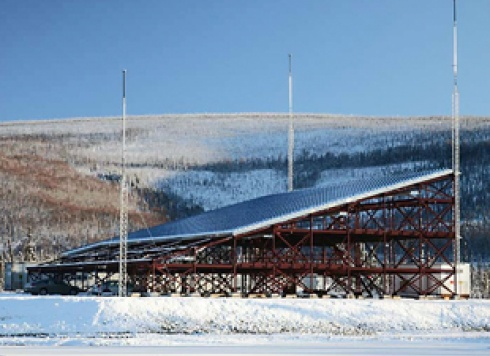
\includegraphics[width=3in]{amisrimage}
\caption{Image of the PFISR \cite{SRIpage}}
\label{fig:amisrpic}
\end{figure}

\subsubsection{Objectives related to 3-D ISR}
There a large number of studies that have used ISR to reconstruct two and three dimensional fields of plasma parameters. Some studies use various types of interpolation to try to stitch together a picture from the one dimensional beams, which give a one dimensional view along range\cite{Semeter2009738,Butler:2013ul,Semeter:2005fo}. Others have taken a tact closer to inverse theory and image reconstruction to create reconstruction of velocity fields of bulk flows or electric fields \cite{butler:imagingfregiondrifts,RDS:RDS20195}. Still, these publications do not get to the core details of reconstructing plasma parameters like the ion and electron temperatures. Interpolations can help visualize the data but these techniques make a lot of assumptions about the underlying imaging process. The goal of this thesis is to present a first principles model of ISR as a three dimensional sensor and use it to create better reconstructions of the plasma parameters.

\subsection{Ionosphere and Phenomena}
The ionosphere is the area of partially ionized gas, or plasma, surrounding the earth, and in a way is like an interface between the earth and outer space \cite{kellybook}. The dynamics of this system are governed by kinetic, fluid and Maxwells equations coupled together \cite{schunk2004ionospheres}. This complicated menagerie of equations allows for the creation of a cornucopia of different phenomena at any number of spatio-temporal scales \cite{Semeter:2008hs,Semeter2009738}.

%In order to understand the behavior of the plasma in the ionosphere one needs to use electromagnetic theory governed by Maxwells Equations seen in Equations \ref{eqn:max1} and \ref{eqn:max2},

%\begin{eqnarray}
%\label{eqn:max1}
%\nabla \cdot \vec{E} = \frac{\rho}{\epsilon_0}\  &&\nabla  \cdot \vec{B} = 0 \nonumber \\
%\nabla  \times \vec{E} = - \frac{\partial B}{\partial t} && \nabla  \times \vec{B} = \mu_{0}\vec{J} +
%\mu_{0}\epsilon_{0}\frac{\partial E}{\partial t}
%\end{eqnarray}
%
%\begin{equation}
%\label{eqn:max2}
%\frac{\partial \rho}{\partial t}+\nabla \cdot \vec{J} = 0
%\end{equation}
% 
%\noindent where $\rho$ is the charge density, $\vec{E}$ is the electric field, $\vec{B}$ is the magnetic field, $\vec{J}$ is the current density, $\mu_0$ is the vacuum permeability and $\epsilon_0$ is the vacuum permittivity. 
%
%In order to close the system of equations often assumptions about the charge density and current density are needed \cite{varnytalk2016}. In the ionosphere though $\vec{J}$ is linked to the electric and magnetic fields, $\vec{E}$ and $\vec{B}$, which are dependent on the particle motion. In the ionosphere these particles move as gas, so to close these systems of equations require the use of fluid and/or kinetic theory depending on what sort of assumptions can be made for the problem.

The study of the Earth's ionosphere is broken up into a number of different regions due to the physical processes that dominate \cite{kellybook}. The demarcations between the D, E and F Regions are based on the altitude, over which various properties of the plasma, including parameters and chemical composition, can greatly vary as shown in Figure \ref{fig:singlefilt} \cite{kellybook}. The regions of the Earth are also parceled out based on the orientation of the magnetic field to the ground and include the high latitude, mid latitude and low latitude regions \cite{schunk2004ionospheres}.

For this thesis most of the focus will be on phenomena from the high latitude F-region. This of special interest due to the number of different phenomena that occur, much of which is due to the perpendicular angle of the Earth's magnetic field to the ground \cite{schunk2004ionospheres}. These phenomena include but are not limited to aurora borealis, polar cap plasma patches and particle precipitation events\cite{Perry:2015jf,Dahlgren:2013ip,dahlgren2012di,Dahlgren:2012dq,semeter:plasmatransport2012}. From a societal standpoint this sort of activity can greatly impact radio propagation and can create interruptions in data services such as the Global Positioning Systems (GPS)\cite{Jiao:2013ei,hunsucker2007high}.


\begin{figure}[!t]
\centering
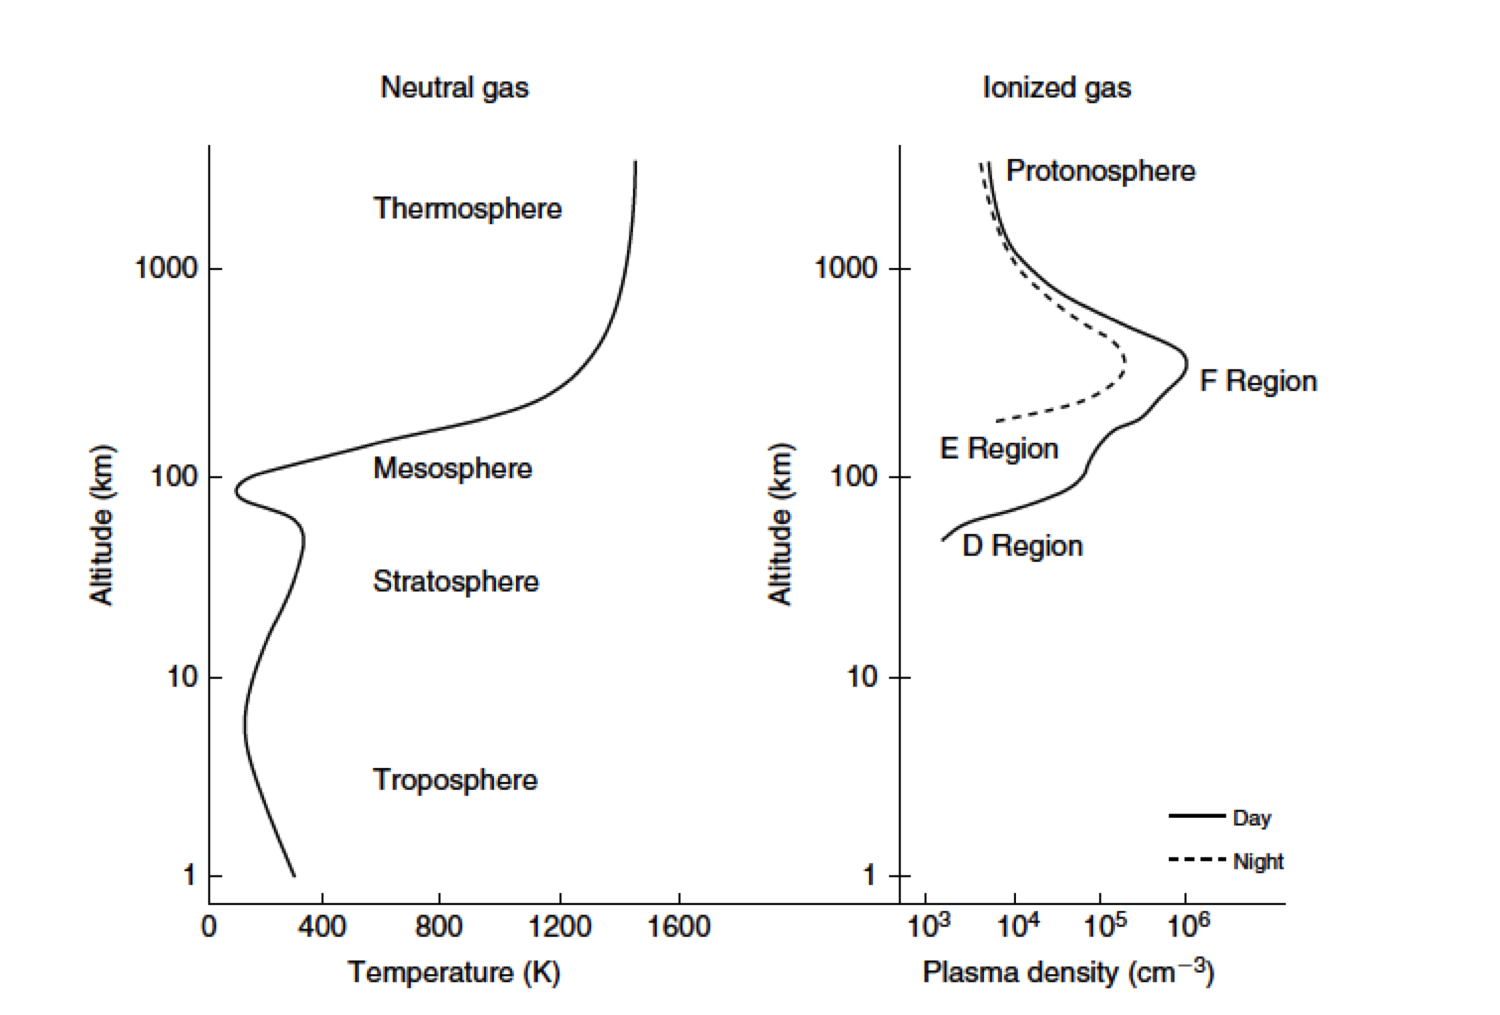
\includegraphics[width=5in]{altvsparams}
\caption{Example profiles of neutral temperature and plasma density from \cite{kellybook}}
\label{fig:singlefilt}
\end{figure}
%These systems right now are all located in what can be considered the high latitude ionosphere.  This is a highly dynamic environment in both time and space.  The plasma can change very quickly due to the physics of the environment.  These types of events can be classified into a number of types that will be of interest to this type of sampling problem.

%\subsubsection{High Spatial Gradient Events}
%Polar cap patches are examples where of high spatial gradients in various plasma parameters \cite{Dahlgren:2012dq,dahlgren2012di}.  In the polar cap large blobs of plasma with elevated electron density travel from the dayside to the night side ionosphere.  These patches can play a large role in plasma transport within the polar ionosphere and interfere with radio transmission as well.  Examples of sensor data that show these patches can be seen in Figure \ref{fig:patches}.
%
%\begin{figure}[!t]
%\centering
%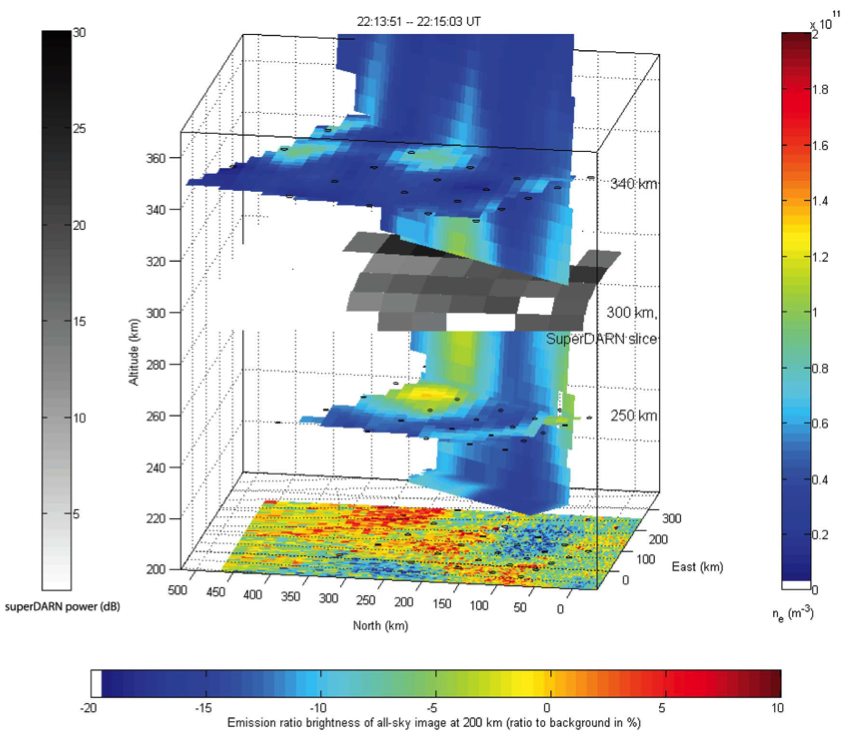
\includegraphics[width=4.0in]{patches}
%% where an .eps filename suffix will be assumed under latex, 
%% and a .pdf suffix will be assumed for pdflatex; or what has been declared
%% via \DeclareGraphicsExtensions.
%\caption{Example of polar cap patches seen in RISR and SuperDARN, from \cite{Dahlgren:2012dq}}
%\label{fig:patches}
%\end{figure}
%
%Large horizontal gradients also occur during geomagnetic storms which can produce large flows.  This can create large disparities in Ion temperature as heating is occurring \cite{Zettergren:2008ba,semeter:plasmatransport2012}.  During these storms ion temperatures can go from 500$^\circ$ K to over 1500$^\circ$ K in the order of kilometers.
%
%These high gradient events can cause some unpredictable errors where two plasma population interface.  These errors can be quite complex due to the nonlinear nature of the inversion process\cite{Vallinkoski1990665}.  Similar behavior has been observed during times of auroral turbulence where shear flows seems to have caused non isotropic temperature measurements\cite{knudsen1993}. 
%%\subsection*{Small Structure Events}
%%\cite{semeter2010CI}
%
%\subsubsection{Dynamic Phenomena}

These phenomena can vary on a multitude of spatio-temporial scales and thus can create difficult sampling problems for sensors tasked measuring them. For the sake of brevity, the rest of the subsection will focus on two examples from the literature and highlight the challenges associated with trying to reconstruct the plasma parameters.

The events shown in \cite{Semeter:2005fo} consist of event known as a poleward boundary intensification (PBI). This occurs when the auroral oval breaks into two separate rings which show a demarcation of different field line configurations in the magnetosphere. The auroral ring closer to the magnetic pole shows a number of strong pulsations which can be seen in both optical and radar data \cite{Semeter:2005fo} .

In the radar reconstruction shown in Figure \ref{fig:Sampling} these events cause large enhancements in electron density that are perpendicular to the ground. These can be challenging to image as these phenomena are moving which can impact how well these events are resolved and ambiguity can be introduced merely in how one processes the data. In this case the researchers found if they integrated fewer pulses per position and allowed for a greater variance in the data they could observe column structuring to the enhancement.

\begin{figure}[htb]
  \begin{minipage}[t]{0.49\linewidth}\centering
    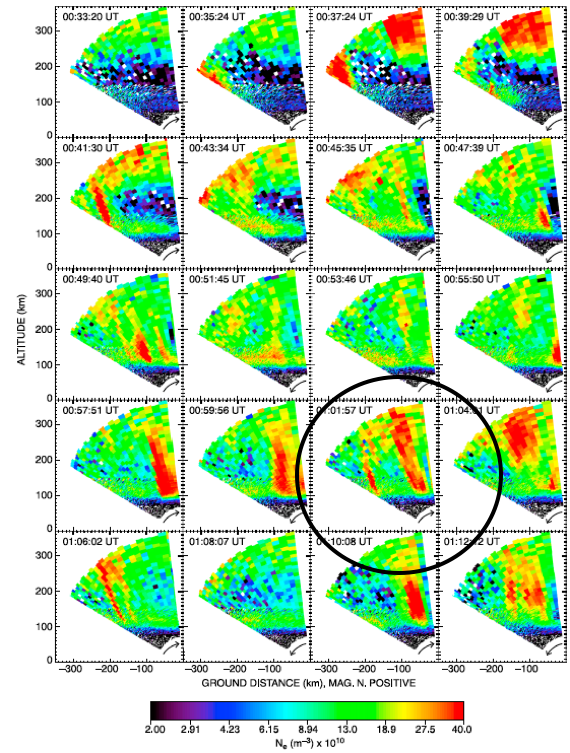
\includegraphics[width=7cm]{pbiall}
    \medskip
    \centerline{(a)}
  \end{minipage}\hfill
  \begin{minipage}[t]{0.49\linewidth}\centering
    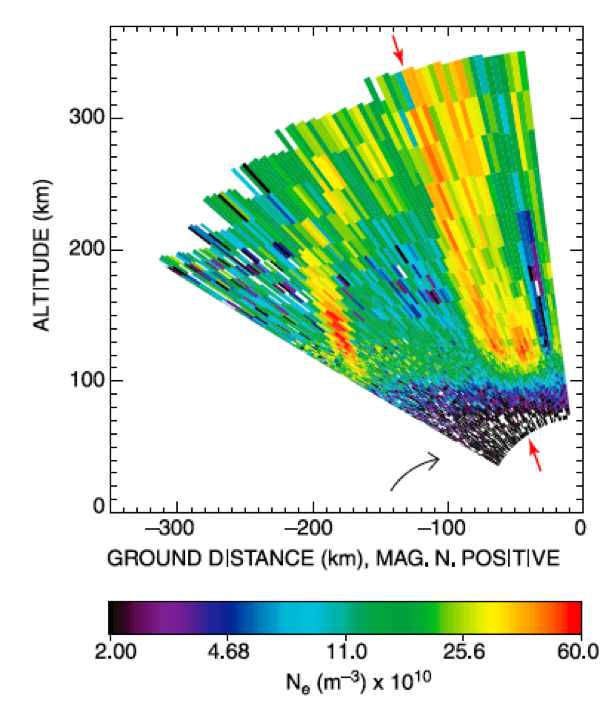
\includegraphics[width=7cm]{pbifast}
    \medskip
    \centerline{(b)}
  \end{minipage}
  \caption{Different views of a poleward boundary intensification event as seen in \cite{Semeter:2005fo}: (a) Data from the Sondastrom processed at 5 seconds; and (b) the same data from the circled frame in b but processed at 2 seconds. }
  \label{fig:Sampling}
\end{figure}

The second phenomena that will be focused on is a sun-aligned auroral arc, specifically from \cite{Perry:2015jf}. These arcs are created by Field Aligned Currents (FAC) from the magnetosphere.The evidence of these structures show themselves in plasma parameters through electron and ion temperature enhancements coincident with electron density depletions next to density enhancements. These structures also are in motion, which can create ambiguities in the measurement process as the plasma moves through the field of view. An example of this type of plasma parameter distribution associated with these types of auroral arcs can be seen in Figure \ref{fig:mzsim}.

\begin{figure}[!t]
\centering
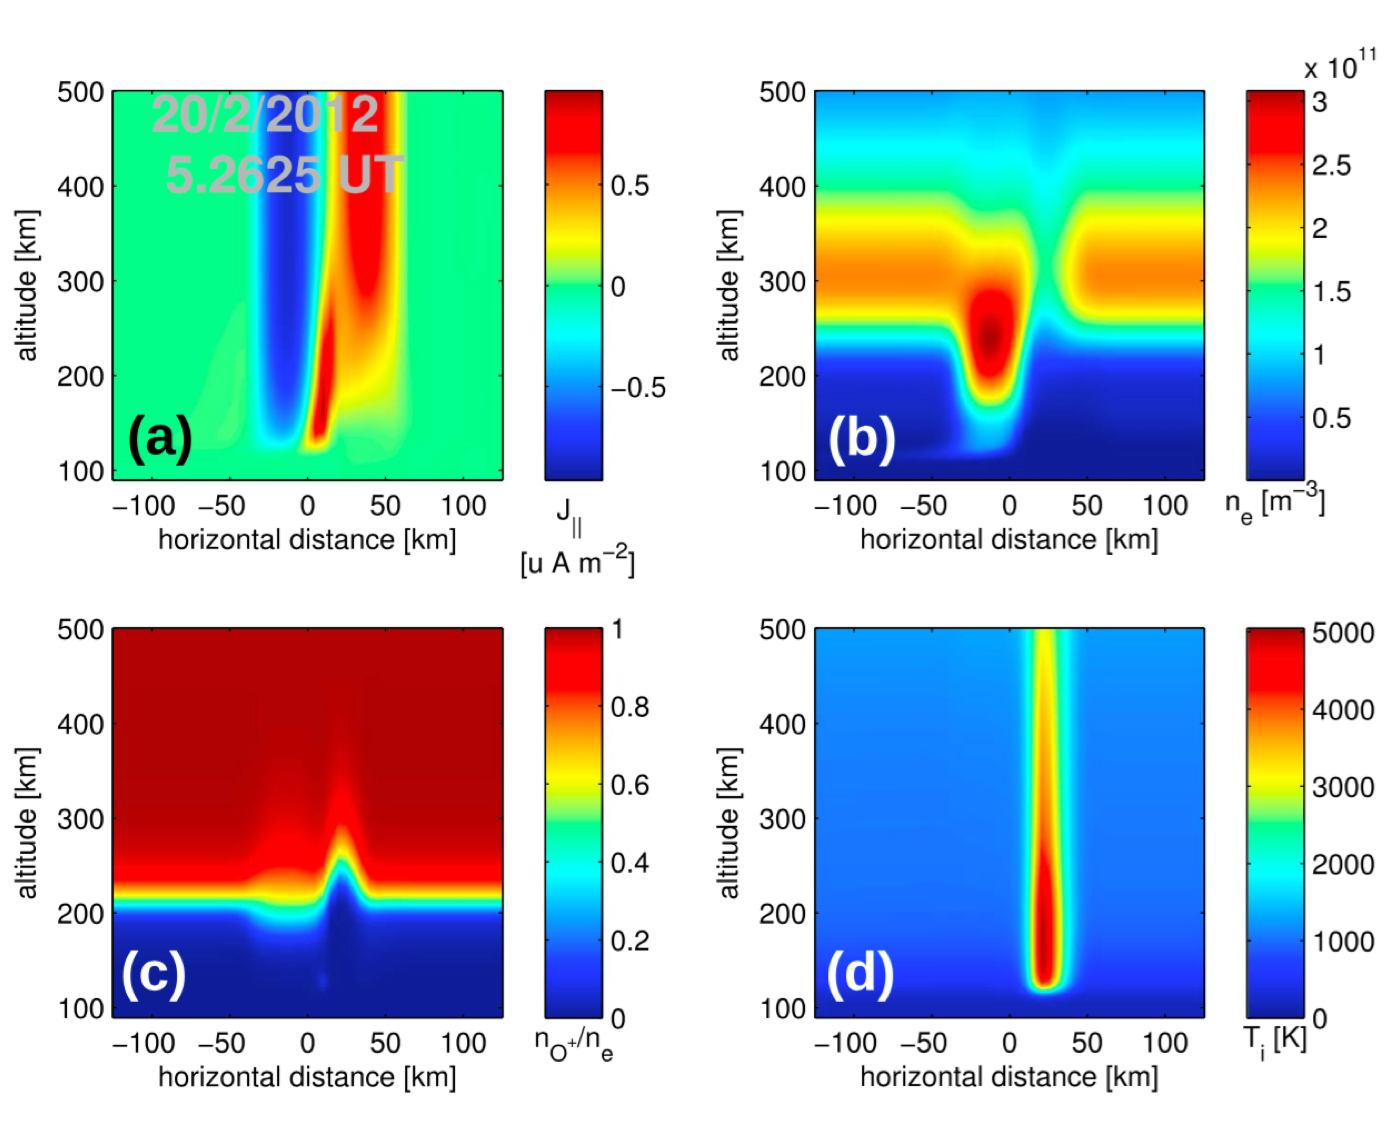
\includegraphics[width=5.0in]{MZsim}
\caption{Image from \cite{Perry:2015jf} showing plasma parameters from a multi-fluid model\cite{semeter:plasmatransport2012} simulating the impact of an auroral arc. }
\label{fig:mzsim}
\end{figure}
%There are also a large number of dynamics and structure found in many auroral events. Using the AMISR system to create volumetric reconstruction of the electron density \cite{Semeter2009738} helped show variability of these events. Figure \ref{fig:eregionact} shows an example of one of these reconstructed events.  Again the like before the researchers again showed the variability during these events by changing the number of pulses integrated and found a large difference in the visible structure.
%\begin{figure}[!t]
%\centering
%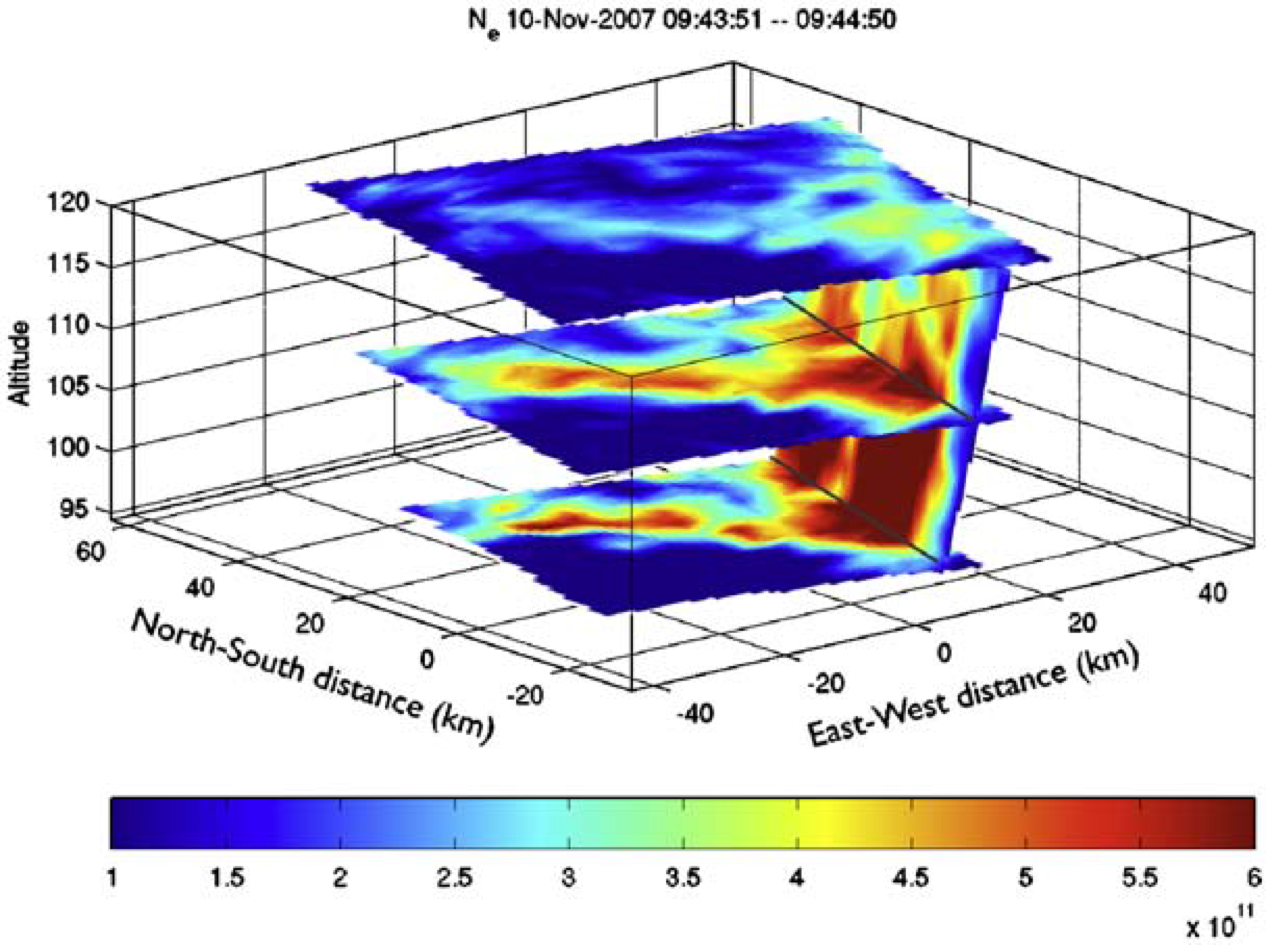
\includegraphics[width=4.0in]{threedamisr}
%\caption{A volumetric reconstruction from AMISR system, from \cite{Semeter2009738}. The reconstruction is of the E-region ionosphere during a auroral precipitation event i.e. electrons following the magnetic field lines of the earth to the lower ionosphere and creating ionization.}
%\label{fig:eregionact}
%\end{figure}
%\subsubsection{High Speed Events}
%At times the ionosphere can be come locally unstable this can create a number of different types of turbulent events. Langmuir turbulence can create coherent structures that will be detected by ISR systems \cite{akbari:2013lt}.  These structures change on the order of one pulse repetition interval of the radar.
%
%Resolving these high speed events are of great interest but also a challenge.  In ISR systems each pulse is used as a sample of a spectral averaging procedure.  It is assumed that these spectrums are identical independent samples.  If spectrum changes during this time, errors in the measurement could take place.  These errors are often unpredictable due to the nonlinear fitting used to fit the spectrum with the plasma parameters.
 %\cite{Dahlgren:2013ip}
%In the past researchers have studied errors associated with different plasma distributions mixing together.  These errors can be quite complex due to the nonlinear nature of the inversion process\cite{Vallinkoski1990665}.  Similar behavior has been observed during times of auroral turbulence where shear flows seems to have caused non isotropic temperature measurements\cite{knudsen1993}. 
\subsubsection{Objectives related to the Phenomena of the Ionosphere}
The main goal of using ISR is to get the most accurate reconstructions of plasma parameters possible. This research creates a framework with which researchers can use to improve their experiment planning. This frame work includes a simulator that can create synthetic ISR data which they can use to try different experiment set ups and reconstruction methods. The simulation examples parameter distribution derived or directly from those shown in Figures \ref{fig:Sampling} and \ref{fig:mzsim} as phantoms to test the reconstruction methodology.

\subsection{Image Reconstruction}
\label{sec:imgrec}
Inverse theoretic image reconstruction gives engineers and scientists a robust frame work to determine the state of system parameters given a data set. This sort of frame work has been applied to numerous problems in science and engineering from X-Ray computed tomographic scanning \cite{kak1988principles} to synthetic aperture radar \cite{1456966}. In this thesis we will use this framework and techniques to improve the quality of the plasma parameter estimates from ISR.

The main gaol of image reconstruction and inverse theory is to reconstruct a set of parameters given a set of data using knowledge of the forward model. Using the notation found in \cite{menke2012geophysical} a general inverse problem can be stated as follows,

\begin{equation}
\label{eqn:invprob}
\mathbf{d}=\mathbf{g}(\mathbf{m})
\end{equation}

\noindent where $\mathbf{d}$ is the data $\mathbf{g}$ is the operator that changes the parameters $\mathbf{m}$ to the data space. 

Although Equation \ref{eqn:invprob} gives a general framework this problem can be difficult to solve. Often, techniques used to solve inverse problems entail some assumption that can be made about the operator $\mathbf{g}$ such as linearity or that its well-posed \cite{0266-5611-4-4-010}. Still there are ways to get around this by doing things such as adding constraints or regularization to the inversion method \cite{Vogel:2002:CMI:581830}.

ISR has in past been presented in this format, although this has mainly been for the case of a single beam \cite{Vierinen:2012ve}. ISR can be thought of a general inverse problem because of the non-linear operation that brings the plasma parameters to the ACF space. Two schools of thought have emerged which in the community on how to be constrain these inversions. The first, full profile analysis, uses plasma parameter constraints, which can give physical constraints to the inversion thus improving the outcome \cite{hysell2008,RDS:RDS3308}. The second set of techniques apply constraints on the estimated ACFs \cite{Virtanen:20082vx,nikoukar2008}, which is less expensive computationally but can create ACFs that cannot be created through IS theory.

\subsubsection{Objectives related to the image reconstruction}
This thesis will couch the estimation of 3-D ISR in the language of inverse theory. It will use techniques to improve the accuracy of the reconstruction of plasma parameters.

\subsection{Outline of dissertation}

Chapter \ref{chapter:isrproc} will go into the background into ISR signal processing. This will be begin by developing the basic signal model and show the processing steps between the sampling complex voltages to plasma parameter measurements.

Chapter 3 will show the derivation of space-time ambiguity function. This will allow for the posing reconstruction of the field of three dimensional plasma parameters in the language of inverse theory. 

Chapter 4 contains a discussion of the frame behind the Simulator for ISR (SimISR). This simulator can create complex voltages and process the data. This can help plan experiments the future. This will also include the examples of simulated data to show the capabilities of this framework.

Chapter 5 will detail an inversion method that has been developed to reduce the impact of the space-time ambiguity. This inversion method allows for plasma parameter reconstructions along the frame of reference of the moving plasma.

\section{Contributions}
Specific contributions of this research are summarized below.

\begin{enumerate}
\item Development of a theoretical framework for the forward model of 3-D ISR plasma parameter reconstructions.
\item Creating a framework full simulation of an ISR system that can which yield synthetic complex voltages.
\item A software package, named SimISR has be derived from previously mentioned simulation framework has been made available to other researchers.
\item A detailed analysis of the simulation framework using SimISR.
\item A new method for inverting the forward model for 3-D ISR plasma parameter reconstructions.
\end{enumerate}
\cleardoublepage

% -------------------------------------
% CHAPTER 2: THE BODY OF THESIS
% -------------------------------------
\chapter{Incoherent Scatter Radar Processing}
\label{chapter:body}
\thispagestyle{myheadings}

% set this to the location of the figures for this chapter. it may
% also want to be ../Figures/2_Body/ or something. make sure that
% it has a trailing directory separator (i.e., '/')!
\graphicspath{{2_Body/Figures/}}

%%%%%%%%%%%%%% Intro %%%%%%%%%%%%%%%%%%%%%%%%%%%%%%%%%%%%%

Radar is common remote sensing modality which has found diverse uses ranging from being used by police to monitor the speed of traffic \cite{richards2010principles}, to mapping the surface of planets in our solar system \cite{campbell2002radar}. The term radar itself is an acronym for radio detection and ranging, which the basic premise of these systems. These systems radiate electro-magnetic waves which reflect off of a target. These reflected waves are then received and processed by the system \cite{skolnik2008radar}. The radar system measures the range $R$, or the distance between the target and sensor, by simply measuring the round trip time $\Delta T$ and using the following conversion,

\begin{equation}
\label{eqn:range_intro}
R=\frac{c\Delta T}{2}
\end{equation}

\noindent where $c$ is the speed of light \cite{richards2010principles}.




The main way to look at Doppler in hard-target radar is to assume it is a multiplication of the radar signal $s(t)$ with a simple single complex exponential

\begin{equation}
\label{simpledop}
s_d(t) = s(t)e^{j\omega_d t},
\end{equation}
 
\noindent where $\omega_d$ is the Doppler frequency of the target or object.  If we say have multiple targets each with their own Doppler frequency and their own weighting, which would represent a relative scattering to each components,  we can represent that signal as the following

\begin{equation}
\label{multiDop}
\displaystyle s_d(t) = \sum_{n}^{N} s(t)X(\omega_n)e^{j\omega_{n} t}.
\end{equation}

\noindent Extending this to a continuum of signals each at each Doppler frequency this becomes

\begin{equation}
\label{conDop}
s_d(t) = \int s(t) X(\omega)e^{j\omega t}.
\end{equation}
\noindent Pulling the $s(t)$ term out of the integral we can see that we are taking the Fourier transform of this relative weighting between each of the scatters and then multiplying it with the signal.  Using simple Fourier properties we can see that this equivalent to a convolution in frequency space of the spectrum of the original radar signal and the Doppler spectrum with the collection of targets.  

The final form of the signal spectrum with Doppler added can be shown as the following

\begin{equation}
\label{finalDop}
s_d(t) = \int \left[\int S(\lambda)X(\lambda-\omega)d\lambda\right] e^{j\omega t}d\omega.
\end{equation}

\noindent This shows that the measured Doppler on the radar signal can be formulated as the convolution of the Fourier transform of radar's signal along with the Doppler spectrum of the target.

\section*{Applying the Model To Pulse Doppler Radar}

In pulse-Doppler (PD) radar a succession of pulses are sent out modulated by the carrier frequency $f_c$.  Each pulse scatters off of the target and which imparts a Doppler frequency $\omega_d = 2\pi f_c \frac{2v}{c}$, where $v$ is the target velocity and $c$ is the speed of light.  This representation of the Doppler frequency is only valid if the target is non-relativistic.  In the case where we are looking at a single target the return of the $m^{th}$ pulse can be represented in the following way\cite{richards:fundamentalsigproc}

\begin{equation}
\label{pdpulse}
y(t) =  A(t)e^{j\phi}e^{j\omega_dmT},
\end{equation}

\noindent where $T$ is the pulse repetition interval (PRI).  In this case each pulse is sampling the Doppler spectrum at a rate of the pulse repetition frequency (PRF).  Using traditional PD processing the PRF determines the maximum unambiguous Doppler frequency.  For example if one wants a system with a carrier frequency of 10 GHz that will resolve a target going the speed of sound with aliasing in Doppler (approximately 340 m/s) that system must have a PRF greater than 45 kHz if one uses the Nyquist theorem.   

To get the final measurement of this spectrum often a Discrete Fourier transform is applied.  When the data arrives to the radar it is sampled in to specific range gates and pulse samples.  Pulse compression is applied across range to help to localize the signal in range.  This operation is basically applying a filter that is the time reversed conjugate of the base band pulse.  After pulse compression operation Discrete Fourier Transforms are taken across the pulse dimension in each range bin.   The final result is commonly referred to as a range-Doppler map.


%%%%%%%%%%%%%%%%%%%%%%%%%%%%%%%%%%%%%%%%%%%%%%%%%%
\subsection{Applying the model to ISR}
In some radar modalities the system is attempting to measure numerous targets.  The number of targets grows the scatters resemble more of a distribution than a single scatterer.  In the case of ISR the radar is trying to sample the velocity spectrum of the distribution of electrons in the upper atmosphere and ionosphere.  

In ISR the goal of the system is often to sample what is called the ion-line spectrum.  From Dougherty and Farley's 1960 paper \cite{dougherty:farley1960} the normalized spectrum can be formulated as 

\begin{equation}
\label{ionline}
X(\theta) = \frac{e^{-\theta^2}}{\pi \theta^2 e^{-2\theta^2}+(2-I(\theta))^2},
\end{equation}

\noindent where $\theta=(\omega/k)\sqrt{m_i/(2KT_i)}$, $K$ is Boltzman's Constant and $I(\theta)$ can be represented as the following:
\begin{equation}
\label{Ifunc}
I(\theta) = 2\theta e^{-\theta^2}\int_0^\theta e^{t^2}dt.
\end{equation}

% make ISR spectra


One can see in this formulation that the distribution is actually dependent on the thermal velocity of the ions $\sqrt{2KT_i/m_i}$.  If one multiplies this velocity by the wavenumber $k$ of the radar we actually get a Doppler frequency.  This term is basically a normalization of the frequency space of the distribution to what would be the Doppler of the average thermal speed.  The distribution $X(\theta)$ is basically the distribution of the scatterers at these different speeds.

To sample this spectrum one needs a process that can sample this frequency response.  Although the function in Equation \ref{ionline} has a number of assumptions built in one could still use it as a way to get a feel for what type of sampling frequencies are required.  If we look at Figure \ref{ionlinefig} we can see it seems to have no appreciable content beyond $3\omega_\theta$, thus one needs a sensor that can sample at a frequency of at least $6\omega_\theta$ if we are using the Nyquist theorem.  To give a rough example we can say that one wants to look at hydrogen ions at a  temperature 600 Kelvin with a sensor that has a center frequency of 450 MHz \footnotemark[1].  This will yield an $\omega_\theta/2\pi$ of about 2 kHz and in order to sample that spectrum one would need to sample at about 12 kHz just to get this spectrum.
  
\footnotetext[1]{This is a very simple example and probably not best for the ionosphere.  I probably should use Oxygen ions or some other species for this example.}

If one were to use a pulse-Doppler sort of approach to sampling the process used in the previous example one would need a PRF of about 12KHz.  This PRF would only allow the pulse scatter off of a targets that are no more farther then 125km out.  This would not work for ionosphere measurement when one want to measure out 700km. 

In order to measure this spectrum ISR systems often use an intra-pulse autocorrelation method to measure the Ion-line spectrum.  To do this a pulse with a long time width is sent.  The length is often on the order of a number of range bins.  It is assumed that the plasma from different range's is uncorrelated but since the pulse is longer than a range bin energy scattered from other ranges are summed into other range bins.  Once the correlations are formed a Fourier transform is taken of the autocorrelation functions (ACF), thus yielding a power spectrum for each range.  This operation can also be described in terms of a Wigner-Ville distribution in that we are taking the Fourier transform of a time dependent correlation.\footnotemark[2] This spectrum is again the Doppler spectrum of the distribution of targets though and one is left with a range-Doppler map.

In a sense pulse-Doppler and ISR are attempting to measure the same quality, a Doppler spectrum of some target but they just have different measurement methods.  In PD radar the Doppler spectrum is measured across the pulses while in ISR the Doppler spectrum is measured within the pulse itself.  

This is mainly because of what the different systems are trying to measure.  In most PD systems the required sample rate of the Doppler does not cause high enough PRFs to cause range ambiguities.  Also in detection systems where point targets are being detected range (and Doppler) ambiguities can often be corrected.

In ISR the target being observed is a distribution of scatterers with a fairly large Doppler bandwidth.  The large Doppler bandwidth along with the need to measure parameters at far ranges requires one to develop the Doppler spectrum using information that is available within a pulse.  The pulses themselves are basically used as samples in an averaging of the autocorrelation function to develop a statistically significant representation of the spectrum.
\footnotetext[2]{ I need to work on the wording of this paragraph and add examples}
\section{Introduction}
Incoherent scatter radar (ISR) is a powerful tool for exploring the ionosphere. These systems can give measurements of electron density $N_e$, ion temperature $T_i$, electron temperature $T_e$, ion velocity $V_i$ and other plasma parameters \cite{dougherty:farley1960, farleydougherty:ISR2, doughteryfarley:ISR3, hagfors1961}. These parameters are measured by matching radar measured power spectra to a parameterized first-principles, physics based model of the power spectrum of the signal scattered from random ionospheric electron density fluctuations. Alternatively, fitting can be done in the lag domain by using the intrinsic autocorrelation function (ACF) of the plasma, which can be determined by taking an inverse Fourier transform of the power spectrum\cite{Lehtinen1996435}. 

The spectral measurement process is fundamentally an estimation of a second order statistic of an inherently random process from the scattering of electrons. In order to get an estimate of the ACF with reasonable statistical properties, an ensemble average must be performed by averaging power spectra or autocorrelation functions together from different pulses. With traditional dish antennas, ISR systems build  statistics in a limited number of ways. One method consists of pointing the radar beam in a specific direction and dwelling until enough pulses are integrated to get the desired statistics. Alternatively, the beam can be scanned through a field of view, collecting pulses while moving. These techniques use an implicit assumption about the uniformity of the plasma parameters within a volume defined by the pulse shape and solid angle beam properties while pulses are being integrated. This leads to an assumption of stationarity of the ACF within a temporal and spatial resolution cell of the radar. 

In many cases, especially in the high latitude ionosphere, this stationarity assumption is not met. Phenomena such as polar cap patches can drift at greater than 1 km/s, and thus the residency time of a particular plasma parcel within a radar beam may be much shorter than the integration time required to estimate an ACF \cite{dahlgren2012di}. In the auroral zone, ionospheric variations produced by auroral particle precipitation occur on similarly short time scales compared to the integration period \cite{Zettergren:2008ba}.

Recently, electronically steerable array (ESA) technology has started to be leveraged by the ISR community. The Advanced Modular Incoherent Scatter Radar (AMISR) systems have already been deployed both at the Poker Flat Alaska (PFISR) and Resolute Bay Canada (RISR) geospace facilities. The European led EISCAT-3D project is currently being developed using phased array technology as well and will be capable of multistatic processing. These new systems are already being used in a number of different ways including creating volumetric reconstructions of plasma parameters \cite{Semeter2009738, Nicolls:2007ie, dahlgren2012di,Dahlgren:2012dq}. These reconstructions primarily consist of recasting ISR data into a Cartesian space through interpolation, after parameters have first been fit in a spherical coordinate system. Others have reconstructed full vector parameters using estimates of the ion velocity which can be determined using the Doppler shift of spectra \cite{butler:imagingfregiondrifts,RDS:RDS20195}.

These new ESA based systems differentiate themselves from dish antennas in a fundamental way. Instead of dwelling in a single beam or scanning along a prescribed direction, an ESA can move to a different beam position within its field of view on a rapid, pulse by pulse basis. An illustration of the differences between ESA and conventional radar systems with respect to statistical integration of radar pulses, focusing on time history of beam positions, starts with the desired grid of geographic parameter coverage in Figure \ref{fig:bp1}. Figure \ref{fig:dbsts} shows a possible path for a dish based antenna to cover this measurement space through moves to different beam positions through time, represented on the z-axis as pulse repetition intervals (PRIs). The dish sweeps through the field of view in a continuous scan.  In contrast, an ESA system can instead move from position to position in discrete steps as seen in Figure \ref{fig:phbsts}. We note as well that the phased array antenna is able to collect data from different beams during overlapping time periods, creating a lattice like pattern. This type of pulse-to-pulse beam position change is very difficult to accomplish with dish antenna systems having significant pointing inertia. 

%\begin{figure}
%	\centering
%	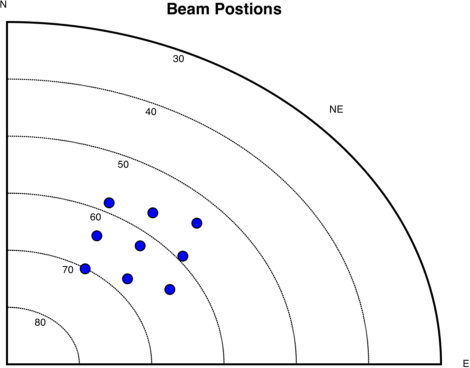
\includegraphics[width=3.5in]{beampositionssts}
%	\caption{A 3x3 grid of desired measurement positions in a
%         hypothetical geodetic latitude/longitude space. }
%	\label{fig:bp1}
%\end{figure}

%\begin{figure}
%	\centering
%	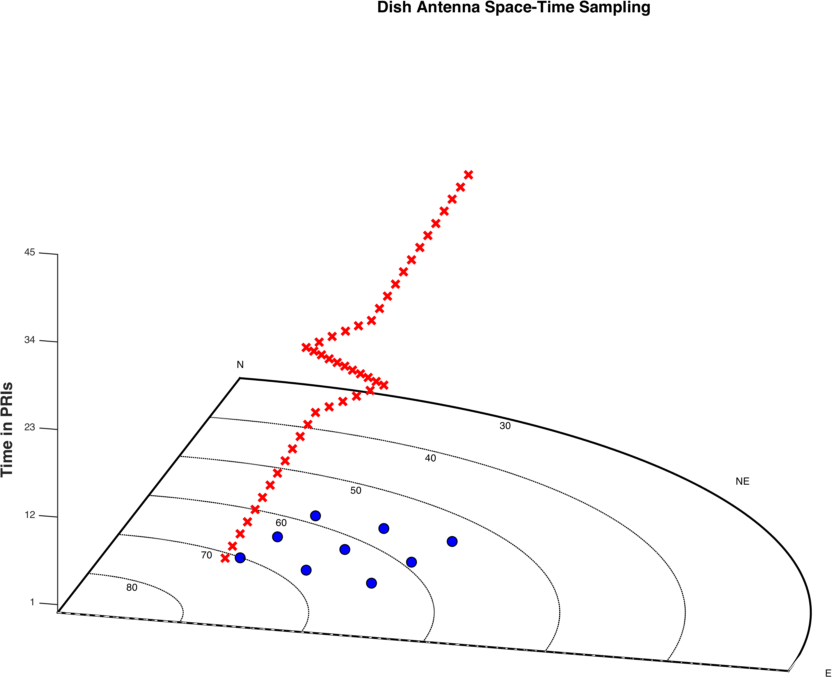
\includegraphics[width=5.5in]{dishsts}
%	\caption{Space-time sampling of the measurement space from Figure~\ref{fig:bp1} using a dish based antenna, where the red x's mark the pulse in beam space and time. Beam positions from Figure \ref{fig:bp1} are shown below in blue at $z=0$.}	
%	\label{fig:dbsts}
%\end{figure}

%\begin{figure}
%	\centering
%	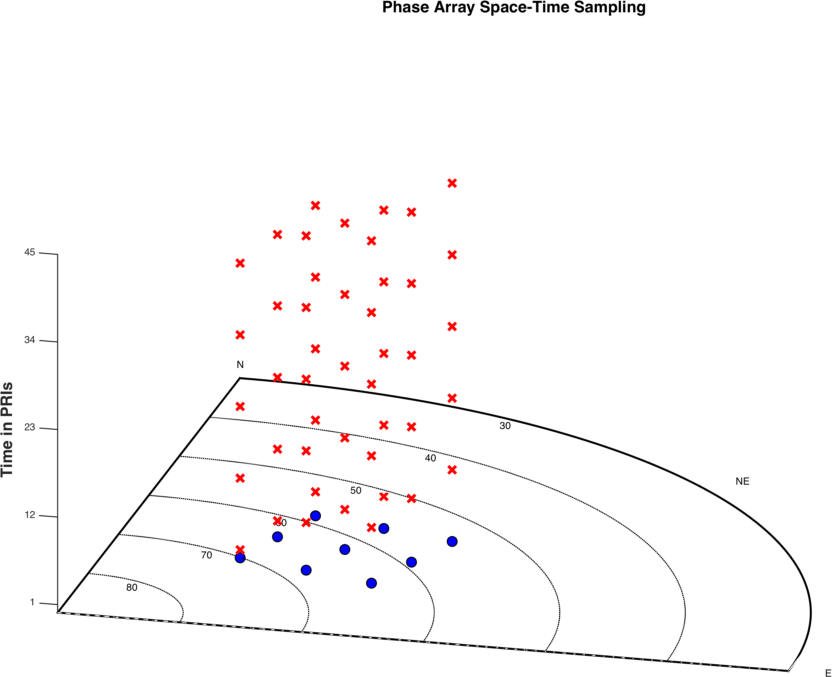
\includegraphics[width=5.5in]{phasedarraysts}
%	\caption{Space-time sampling of the measurement space from Figure~\ref{fig:bp1} using a phased array based antenna, where the red x's mark the pulse in beam space and time. Beam positions from Figure \ref{fig:bp1} are shown below in blue at $z=0$.}	
%	\label{fig:phbsts}
%\end{figure}

The rapid steering ability of ESA systems relative to space-time sampling yields a new flexibility, in post processing, to statistically combine information from different beams using knowledge of the plasma velocity field, where this information is obtained either from external sources or from the Doppler shift of the ionospheric echoes themselves. This can help to relax the assumption of stationarity for plasmas that are evolving or changing their shape on time scales longer than the integration time. If the plasma moves into a different beam, returns from the same plasma can be integrated together with proper bookkeeping. This is contrary to the situation with dish antennas where returns from multiple plasma populations with different parameter sets are unavoidably averaged together.

In order to take advantage of new ESA flexibilities, this work puts forth the idea of the space-time ambiguity function. This concept extends the range ambiguity to all three spatial dimensions along with time. The goal of this paper is to develop a new formalism for treating space-time ambiguity for electronically steerable ISRs, and in particular ISRs that are capable of sampling a given volume on a pulse-by-pulse basis.   This paradigm can also be applied to other types of ISR system designs as well, but much of the utility of using this new formalism is more straightforwardly realized with ESA based systems.  An outline of the paper's development is as follows.  After developing the ambiguity formalism, we will develop specific cases of the impact of the three-dimensional ambiguity on moving plasma using conditions characteristic of polar cap patches. A simulation of a polar cap patch using a full ISR simulator, which creates ISR data at the I/Q level, will be shown. Lastly we will briefly discuss strategies that could improve measurements from electronically steerable ISR systems.

%%%%%%%%%%%%%% Ambiguity Derivation%%%%%%%%%%%%%%%%%%%%%%%%%%%%%%%

\section{Space-Time Ambiguity}

The space-time ambiguity can be thought of as a kernel to a combined volume and time integration operator. In the derivations that follow, we show that this ambiguity can be represented as a kernel operator in a Fredholm integral equation:

\begin{equation}
\label{eqn:friedholm}
\rho(\tau_s ,\mathbf{r}_{s},t_s) = \int L(\tau_s, \mathbf{r}_{s},t_s,\tau,\mathbf{r},t) R(\tau,\mathbf{r},t) dVd t d\tau
\end{equation}

\noindent where, for ISR, $L(\tau_s, \mathbf{r}_{s},t_s,\tau,\mathbf{r},t) $ is a blurring kernel over time and space, and $R(\tau,\mathbf{r},t) $ indicates the plasma medium's autocorrelation function at the lag $\tau$, time $t$, and position $\mathbf{r}$.

By using this formulation, many parallels between ISR and classic camera blurring problems can be made. In cameras, blurring can take place when an object moves over a space covered by one pixel while the shutter is open and the CCD is collecting photons. A diagram of this can be seen in Figure \ref{fig:ccd}. The same holds for the ISR measurement problem, except that the pixels are no longer square or continuous in Cartesian space and instead are determined by the beam shape and pulse pattern. This is shown in the diagrams in Figure \ref{fig:radarblur}.


%\begin{figure}[h!]
%\centering
%	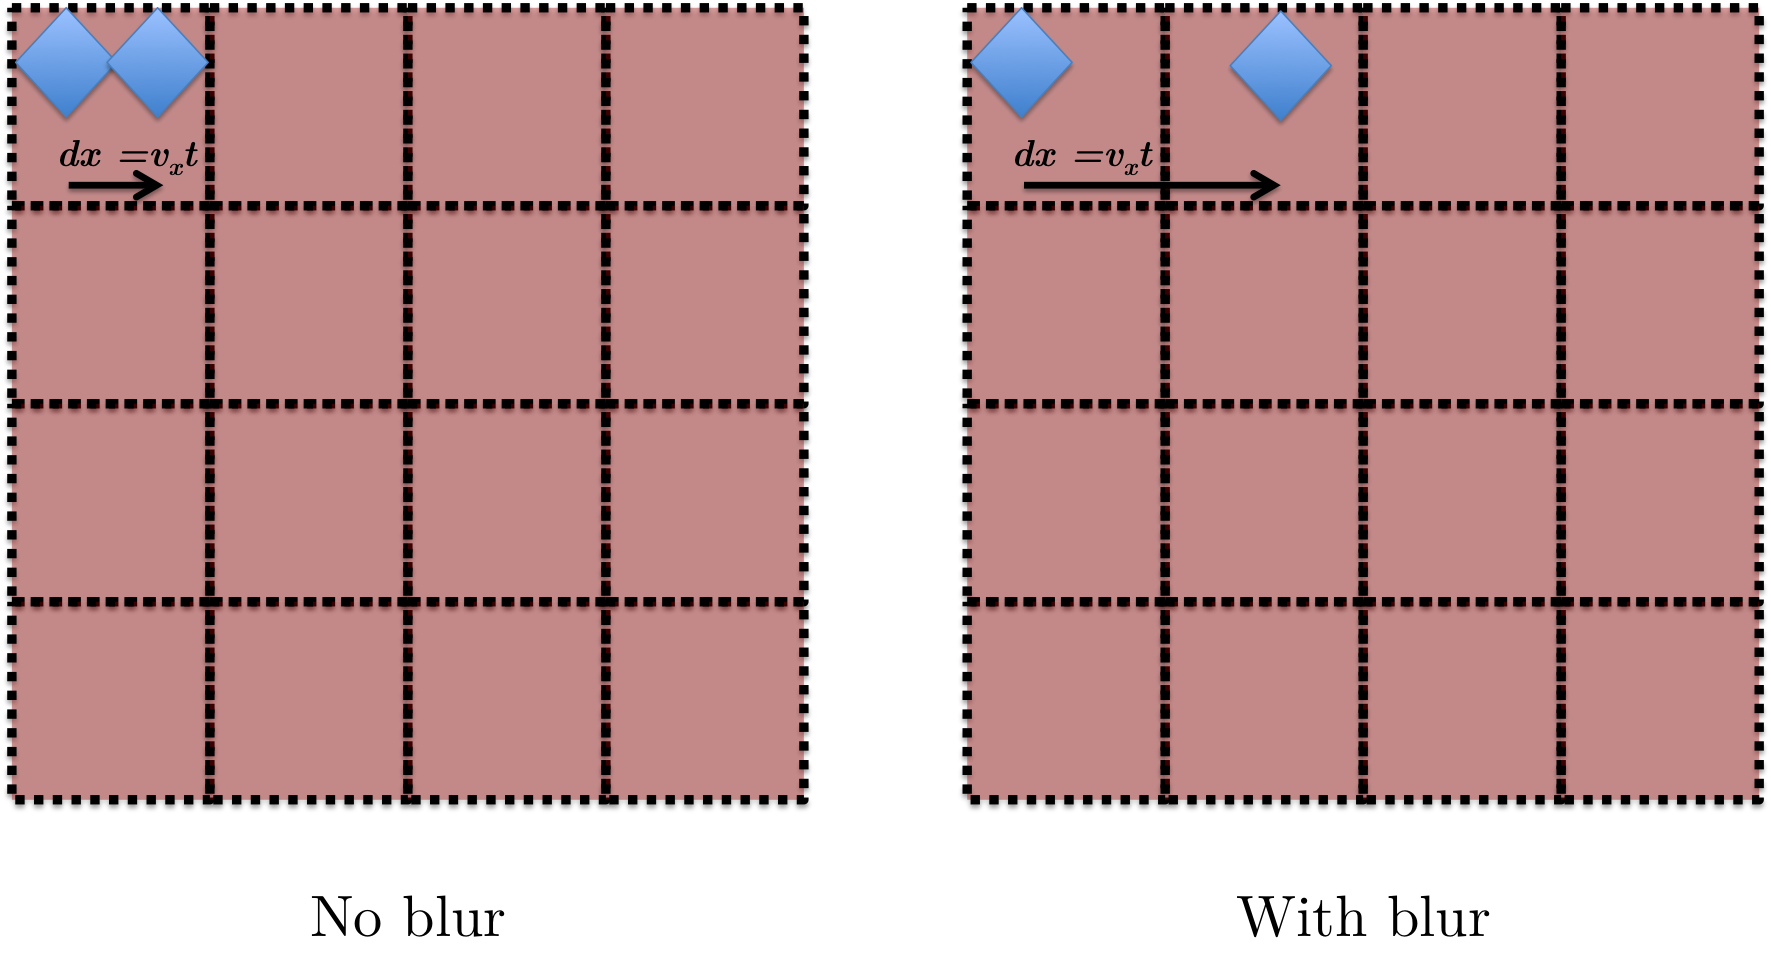
\includegraphics[height=3in]{ccddiagramall}
%	\caption{CCD resolution cell diagram, showing cases where an object will be properly resolved and be blurred.}
%	\label{fig:ccd}
%\end{figure}

%\begin{figure}[h!]
%\centering
%	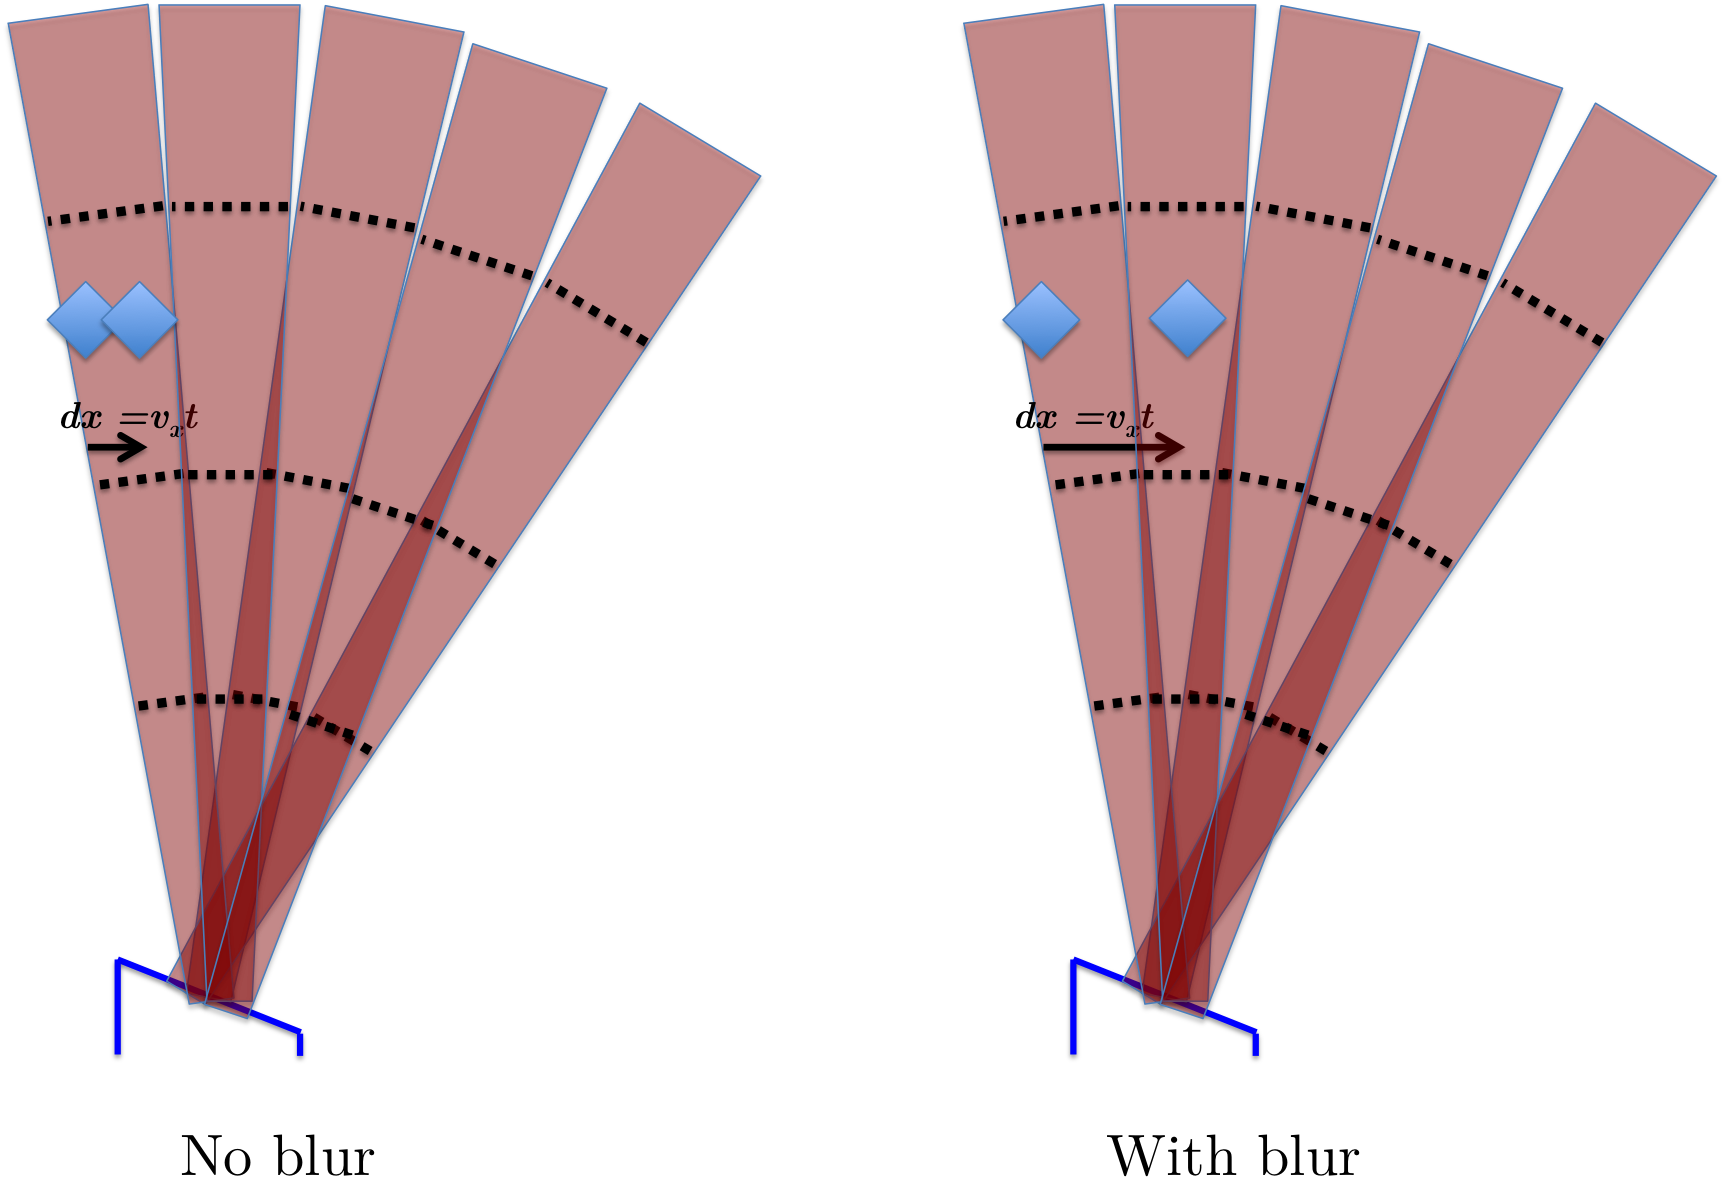
\includegraphics[height=3in]{radardiagramall}
%	\caption{ISR resolution cell diagram, showing cases where an object will be properly resolved and be blurred.}
%	\label{fig:radarblur}
%\end{figure}

\subsection{Coordinate System Definitions}

Before we derive the full space-time ambiguity function, $L(\tau_s,\mathbf{r}_s,t_s,\tau,\mathbf{r},t)$, we will start with defining our coordinate system.  Our three dimensional coordinate system is defined as $\mathbf{r}=[x,y,z]^T$. For this coordinate system, $\mathbf{r}=[0,0,0]^T$ at the location of the radar and thus $r=|\mathbf{r}|$, also known as the range variable. This allows for the use of polar coordinates $\mathbf{r} =  [r,\theta_,\phi]^T$ where $\theta$ and $\phi$ are, respectively, the observer's elevation and azimuth angles.

The radar samples this space at a set of discrete points which will be referred to as $\mathbf{r}_s = [x_s,y_s,z_s]^T$ along with the discretized range expression $r_s=|\mathbf{r}_s|$. The sampled space consists of a number of points, composed of range gates within a beam multiplied by the number of beams. These points can also be referred in polar coordinates $\mathbf{r}_s = [r_s,\theta_s,\phi_s]^T$, where $\theta_s$  and $\phi_s$ are, respectively, the observationally sampled elevation and azimuth angles.

For notation purposes, we use two different sets of time commonly known in the hard-target radar literature as fast-time, $n$ and slow-time, $t$ \cite{richards:fundamentalsigproc}. Fast-time is used to describe processes with correlation time less than one PRI. Slow-time will be used for processes that decorrelate in time on the order of, or longer than, the system's PRI. In order to form estimates of ACFs with desired statistical properties, it is assumed that the plasma parameters parameters will change on the order of many tens to hundreds of PRIs in their stationary reference frame (i.e. remain wide sense stationary for this time). Generally, for incoherent scatter applications in the E-region of the ionosphere ($\approx$100 km altitude) and above, the decorrelation time is less than a PRI for systems with a center frequency in the UHF band, and thus ACFs must be formed over fast-time.

The terms $n$ and $t$ represent continuous variables, while $n_s$ and $t_s$ will be the fast time and slow time parameters sampled by the radar. The sampling rate of $n_s$ is set by the rate at which the system's A/D converters are run. The sampling of $t_s$ can, at the highest rate, be the PRI. At its lowest rate, it can be sampled once in a non-coherent processing interval (NCPI), or equivalently in a period of time it takes the radar to average the desired number of pulses for each beam. 

\subsection{Derivation}

The physical scattering mechanism underlying ISR produces measurable radar scatter from electron density fluctuations in the ionosphere, $n_e(\mathbf{r},n)$, at a specific wavenumber $\mathbf{k}$. These fluctuations scatter radio waves which can be observed by the receiver system of the radar \cite{dougherty:farley1960}. The emitted radar signal at the transmitter has a pulse shape $s(n)$ modulated at a central frequency creating a scattering wave number $\mathbf{k}$. Using the Born approximation, the signal received at time $n$, $x(n)$, can be represented as the following

\begin{equation}
\label{eq:xt}
x(n) = h(n) \ast \int \exp\left[-j\mathbf{k} \cdot \mathbf{r}\right]  s\left(n-\frac{2r}{c}\right) n_e(\mathbf{r},n) d\mathbf{r},
\end{equation}

\noindent where $h(n)$ is the receiver filter and the $\ast$ represents the convolution operator. In modern ISR systems, this signal $x(n)$ is then sampled at discrete points in fast-time which will be referred to as $n_s$. The convolution and sampling operation can be brought in the integral as the following,

\begin{equation}
\label{ex:xtaug}
x(n_s) = \int \exp\left[-j\mathbf{k} \cdot \mathbf{r}\right]  s\left(n-\frac{2r}{c}\right) n_e(\mathbf{r},n)h(n_s-n) d\mathbf{r}dn
\end{equation}


Once the signal has been received and sampled, the autocorrelation function is then estimated from the sampled signal $x(n_s)$. The full expression of the underlying autocorrelation of this signal is the following, 

\begin{multline}
\label{ex:acf0}
\langle x(n_s)x^*(n_s')\rangle =  \int \exp\left[-j \mathbf{k}\cdot \left(\mathbf{r}'-\mathbf{r} \right)\right]s\left(n-\frac{2r}{c}\right)s^*\left(n'-\frac{2r'}{c}\right) \\ h(n_s-n)h(n_s'-n')\langle n_e(\mathbf{r},n)n^*_e(\mathbf{r}',n')\rangle d\mathbf{r} d\mathbf{r}'dn dn',
\end{multline}

\noindent where $r'$ is the magnitude of the vector $\mathbf{r}'$. By assuming stationarity of second order signal statistics along fast time, we can then substitute the lag variables $\tau\equiv n'-n$, and $\tau_s\equiv n_s'-n_s$. With these substitutions, Equation \ref{ex:acf0} becomes


\begin{multline}
\label{ex:acf1}
\langle x(n_s)x^*(n_s+\tau_s)\rangle =\int \exp\left[-j \mathbf{k}\cdot \left(\mathbf{r}'-\mathbf{r} \right)\right]s\left(n-\frac{2r}{c}\right)s^*\left(n+\tau-\frac{2r'}{c}\right) \\ h(n_s-n)h(n_s+\tau_s-n-\tau) \langle n_e(\mathbf{r},n)n^*_e(\mathbf{r}',n+\tau)\rangle d\mathbf{r} d\mathbf{r}' dnd\tau
\end{multline}

\noindent We can make a simplifying assumption at this point that the space-time autocorrelation function of $n_e(\mathbf{r},t)$, $\langle n_e(\mathbf{r},n)n_e(\mathbf{r}',n+\tau)\rangle$, will go to zero as the magnitude of $\mathbf{y} \equiv \mathbf{r}'-\mathbf{r}$ increases beyond the debye length \cite{farley1969}. Thus, the rate which the spatial autocorrelation goes to zero will be such that $\tau\gg \frac{2||\mathbf{y}||}{c}$, allowing us to set $r= r'$ inside the arguments of $s$ and $h$. This allows Equation \ref{ex:acf1} to be rewritten as 
 
 \begin{multline}
 \label{ex:acf2}
 \langle x(n_s)x^*(n_s+\tau)\rangle = \int s\left(n-\frac{2r}{c}\right)s^*\left(n+\tau -\frac{2r}{c}\right) h(n_s-n)h^*(n_s+\tau_s-n-\tau) \\\left[\int \exp\left[-2j \mathbf{k}\cdot \mathbf{y}\right] \langle n_e(\mathbf{r},n)n^*_e(\mathbf{y}+\mathbf{r},n+\tau)\rangle d\mathbf{y} \right]drdn d\tau.
 \end{multline}

The inner integral is a spatial Fourier transform evaluated at the wave number of the radar $\mathbf{k}$. By again asserting stationarity along fast time, we can represent the true ACF as the following,
 \begin{equation}
 \label{eq:spft}
R(\tau,\mathbf{r})= \langle |n_e(\mathbf{k},r,\tau)|^2\rangle \equiv  \int \exp\left[-2j \mathbf{k}\cdot \mathbf{y} \right] \langle n_e(\mathbf{r},b)n^*_e(\mathbf{y}+\mathbf{r},n+\tau)\rangle d\mathbf{y}.
 \end{equation}
 
 \noindent Now Equation \ref{ex:acf2} becomes
 
 \begin{equation}
 \langle x(n_s)x^*(n_s+\tau_s)\rangle = \int \langle |n_e(\tau,\mathbf{k},\mathbf{r})|^2\rangle\left[\int s(n-\frac{2r}{c})s^*(n+\tau -\frac{2r}{c})h(n_s-n)h^*(n_s+\tau_s-n-\tau) dn \right]d\tau dr.
 \end{equation}

 If $n_s$ is replaced with $2r_s/c$ we can introduce the range ambiguity function $W(\tau_s,r_s,\tau,r)$ by doing the following substitution,
 \begin{equation}
 \label{eqn:rngamb}
 W(\tau_s,r_s,\tau,r)= \int s(n-\frac{2r}{c})s^*(n+\tau -\frac{2r}{c})h(2r_s/c-n)h^*(2r_s/c+\tau_s-n-\tau) dn.
 \end{equation}
 
Assuming, for the moment, that $R(\tau,\mathbf{r})$ only varies across the range dimension $r$, we can now represent this in the form of a Fredholm integral equation
 
 \begin{equation}
 \label{eqn:fredfirst}
 \langle x(2r_s/c)x^*(2r_s/c+\tau_s)\rangle = \int W(\tau_s,r_s,\tau,r)R(\tau,r) drd\tau.
 \end{equation}
 
\noindent The range ambiguity function, $W(\tau_s,r_s,\tau,r)$, can be thought of as a smoothing operator along the range and lag dimensions of $R(\tau,r)$. This result is also derived in \cite{nikoukar2008}, \cite{Woodman:1991is} and \cite{hysell2008}

 
The spatial ambiguity across azimuth and elevation angles is determined by the antenna beam pattern. In phased array antennas, this beam pattern is ideally the array factor multiplied by the element pattern \cite{Balanis:2005:ATA:1208379}. The array factor is determined by a number of things including the element spacing and the wave number of the radar, $k$. For example, by making idealized assumptions with no mutual coupling and that the array elements are simple cross dipole elements, AMISR systems will have the following antenna pattern for pointing angle ($\theta_s,\phi_s$): 

 \begin{equation}
 \label{eqn:amisrpat}
F(\theta_s,\phi_s,\theta,\phi) = \frac{1}{2}(1+\cos(\theta)^2)\left[ \frac{1}{MN} \left(1+\exp\left[j(\psi_y/2 + \psi_x)\right]\right)\frac{\sin((M/2) \psi_x)}{\sin(\psi_x)} \frac{\sin((N/2) \psi_x)}{\sin(\psi_x/2)}\right]^2,
 \end{equation}
 
 \noindent where $\psi_x = -k d_x(\sin\theta\cos\phi-\sin\theta_s\cos\phi_s)$, $\psi_y = -k d_y(\sin\theta\sin\phi-\sin\theta_s\sin\phi_s)$ and $M$ is the number of elements in the $x$ direction of the array, and $N$ is the number of elements in the $y$ direction(see Appendix: \ref{App:AMISRarr} for derivation).


The spatial ambiguity is a separable function made up of the components of $W(\tau_s,\tau,r_s,r)$ and $F(\theta_s,\phi_s,\theta,\phi)$. These two functions can be combined by multiplying the two, creating the spatial ambiguity function  $K(\tau_s,\mathbf{r}_s,\tau,\mathbf{r})$. This yields an expression for a single statistical realization of the ACF of the incoherent scatter random process, which will be referred to as $\rho(\tau_s,\mathbf{r}_s)$:


 \begin{align}
  \label{eqn:volume}
\rho(\tau_s,\mathbf{r}_s) &= \int F(\theta_s,\phi_s,\theta,\phi)W(\tau_s,r_s,\tau,r) R(\tau,\mathbf{r}) dV d\tau ,\\
	&= \int K(\tau_s,\mathbf{r}_s,\tau,\mathbf{r}) R(\tau,\mathbf{r})  dVd\tau.
\end{align}

A rendering of an example of this full spatial ambiguity function for an uncoded long pulse, with antenna pattern from Equation \ref{eqn:amisrpat} for four beams, can be seen in Figure \ref{fig:amb4}.

%\begin{figure}
%	\centering
%	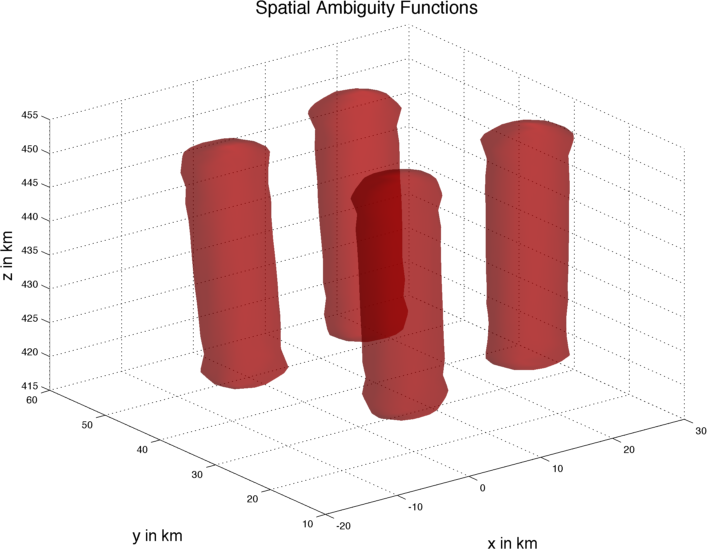
\includegraphics[width=5.5in]{spaceamb}
%	\caption{Full spatial ambiguity function in Cartesian space for case with 4 beams with trailing edge of a 240$\mu$s pulse at 400km range. The surface represents the half power point of the ambiguity function.}	
%	\label{fig:amb4}
%\end{figure}

As mentioned above, this one pulse ACF estimate represents a single sample of a random process. In order to create a usable estimate, multiple samples of this ACF need to be averaged together to reduce the variance to sufficient levels in order to fit the estimate to a theoretical ACF that is a direct function of plasma parameter values. To show the impact of this averaging in creating the estimate of the ACF, we will add slow-time dependence to the expression for the medium ACF, which now becomes $R(\tau,\mathbf{r},t)$, and will also add another separable function $G(t_s,t)$ to the kernel. This function $G(t_s,t)$ can be thought of as a sampling and blurring kernel for the ACF if the plasma parameters change within an NCPI. Since the amount of time that the radar pulse is illuminating the plasma in a point of space is very short compared to the PRI, $G(t_s,t)$ can take the form of a summation of Dirac delta functions 

\begin{equation}
\label{eqn:Gexp}
G(t_s,t) = \displaystyle \sum_{j=0}^{J-1}\alpha_j \delta(t-t_s-jT_{REV}),
\end{equation}

\noindent where $J$ counts the number of pulses used over a NCPI, $T_{REV}$ is the amount of time it takes the radar to revisit the specific beam and $\alpha_j$ represent the weights that the radar assigns to the pulses. For systems using pulse-to-pulse steering, one strategy revisits each beam sequentially, in this case making $T_{REV}=N_{beam}T_{PRI}$, where $N_{beam}$ is the number of beams and $T_{PRI}$ is the PRI time period. For the case where weights are set to $1/J$, this operation simply averages the pulses. With Equation \ref{eqn:Gexp} incorporated into the overall ambiguity we obtain the full integral equation,

\begin{equation}
\label{eqn:sptamb}
	\rho(\tau_s,\mathbf{r}_s,t_s) =\int L(\tau_s,\mathbf{r}_s,t_s,\tau,\mathbf{r},t)R(\tau,\mathbf{r},t)dVdtd\tau.
\end{equation}

\noindent The final kernel, $L(\tau_s,\mathbf{r}_s,t_s,\tau,\mathbf{r},t) = G(t_s,t)K(\tau_s,\mathbf{r}_s,\tau,\mathbf{r})$, encompasses the full space-time ambiguity.

\subsection{Ambiguity after Frame Transformation}

We will now focus on the impact of the motion of plasma as it is going through the field of view of the radar. We will assume that the radar is integrating over a length of time $T$ beginning at $t_s$. The kernel $L$ will be represented as a separable function $K$ and $G$ as in Equation \ref{eqn:sptamb}. In this case, $G$ will be a summation of Dirac delta functions with weights of $1/J$. This will change Equation \ref{eqn:sptamb} to the following:

\begin{equation}
\label{eqn:L2}
\rho(\tau_s,\mathbf{r}_s,t_s) = \int K(\tau_s,\mathbf{r}_s,\tau,\mathbf{r}) \left[(1/J)\int_{t_s}^{t_s+T} \displaystyle \sum_{j=0}^{J-1} \delta(t-t_s-jT_{REV})R(\tau,\mathbf{r},t) dt\right] dVd\tau.
\end{equation}

Of specific interest in this study are instances in the high latitude ionosphere where embedded plasma structures are moving due to electric field drivers applied by the magnetosphere. In this case, it will be assumed that the plasma is a rigid object and will not deform with respect to $\mathbf{r}$ over time period $[t_0,t_0+T]$ where $T=JT_{REV}$ is the time for one NCPI. Also, it will be assumed that the plasma parcel moves with a constant velocity $\mathbf{v}$. Thus $R(\tau,\mathbf{r},t)\Rightarrow R(\tau,\mathbf{r}+\mathbf{v}t)$. The assumption of rigidity can in some cases be valid over the time period of the NCPI, on the order of a few minutes, while the plasma moves through the field of view of the radar. For example, in the high latitude ionosphere, large scale features in structures such as patches decay on the order of hours \cite{Tsunoda:1988ul}. This assumption is useful because it allows our framework to analyze impacts of these plasma variations on the parameter resolution of ISR systems. With these assumptions, Equation \ref{eqn:L2} becomes,

\begin{equation}
\label{eqn:L3}
\rho(\tau_s,\mathbf{r}_s,t_s) =(1/J) \int \int_{t_s}^{t_s+T} \displaystyle \sum_{j=0}^{J-1}\delta(t-t_s-jT_{REV}) K(\tau_s,\mathbf{r}_s,\tau,\mathbf{r})R(\tau,\mathbf{r}+\mathbf{v}t)dtdVd\tau\end{equation}

A change of variables to $\mathbf{r}' = \mathbf{r}+\mathbf{v}t$ acts as a Galilean transform and applies a warping to the kernel, changing the frame of reference. Since $R(\tau,\mathbf{r}')$ is no longer dependent on $t$, Equation \ref{eqn:L3} can be integrated in time and becomes:

\begin{equation}
\label{eqn:L5}
\rho(\tau_s,\mathbf{r}_s,t_s)= (1/J)\int \left[ \;\;  \displaystyle \sum_{j=0}^{J-1} K(\tau_s,\mathbf{r}_s,\tau,\mathbf{r}'-\mathbf{v}(t_s+jT_{REV})) \;\; \right]R(\tau,\mathbf{r}')dVd\tau.
\end{equation}

The problem can now be simplified further back to a Fredholm integral equation by simply replacing the terms in the square brackets as a new kernel $A(\tau_s,\mathbf{r}_s,t_s,\tau,\mathbf{r}')$:

\begin{equation}
\label{eqn:L6}
\rho(\tau_s,\mathbf{r}_s,t_s)= \int A(\tau_s,\mathbf{r}_s,t_s,\tau,\mathbf{r}') R(\tau,\mathbf{r}')dVd\tau.
\end{equation}

\noindent The impact of the plasma velocity on the ambiguity function can be seen in Figure \ref{fig:ambtime}. This is the same ambiguity as seen in Figure \ref{fig:amb4} but with a velocity of 500 m/s in the $y$ direction over a period of 2 minutes. This velocity creates a larger ambiguity function in the frame of reference of the moving plasma.

%\begin{figure}[!t]
%	\centering
%	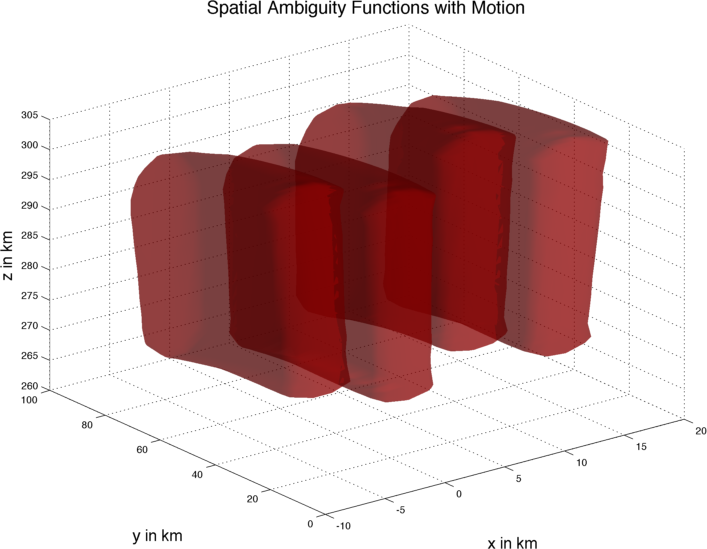
\includegraphics[width=5.5in]{spaceambmoving}
%	\caption{Same spatial ambiguity as in Figure \ref{fig:amb4} but now with 500 m/s velocity in $y$ direction in plasma frame of reference. The surface represents the half power point of the ambiguity function.}
%	\label{fig:ambtime}
%\end{figure}

The operator $A$ can be determined through knowledge of the radar system's beam pattern along with the experiment's pulse pattern, integration time and inherent velocity of the plasma. This velocity $\mathbf{v}$ could be separately estimated by taking measurements of the Doppler shift by using a methodology like that seen in \cite{butler:imagingfregiondrifts}. With this strategy, the operator is now acting purely as a spatial blurring function instead of a full space-time function. We note that reducing dimensionality of the problem can make it easier to solve the inverse problem in practice.

\cleardoublepage

% -------------------------------------
% CHAPTER 3: CONCLUSION
% -------------------------------------
\chapter{Conclusions}
\label{chapter:Conclusions}
\thispagestyle{myheadings}

% set this to the location of the figures for this chapter. it may
% also want to be ../Figures/2_Body/ or something. make sure that
% it has a trailing directory separator (i.e., '/')!
\graphicspath{{3_Conclusion/Figures/}}

\section{Summary of the thesis}

Time to get philosophical and wordy.

IMPORTANT: In the references at the end of thesis, all journal names must be
spelled out in full, except for standard abbreviations like IEEE, ACM, SPIE,
INFOCOM, ...
\cleardoublepage

%\appendix
\begin{appendices}
\chapter{Ionosphere Incoherent Scatter Spectrum}
\label{appendix1}
\thispagestyle{myheadings}
\graphicspath{{Appendix/Figures/}}

%%%%%%%%%%%%%%%%%%%%%%%%%%%%%%%%%%%%%%%%%%%%%%%%%%%%%%%%%%%%%%%%%%%%%%%%%

This is the mathematical basis for calculating incoherent scatter spectrum for a given set of ionosphere state parameters. The appendix uses the methods developed \cite{kudeki:milla:1} and \cite{Kudeki:2006kx}.

\section*{Overall Formulation}
The first step comes from \cite{kudeki:milla:1} where a lumped circuit model is used to describe the spectrum. In it the independent thermal fluctuations of each species of ions and electrons are treated as current sources and the macroscopic conductances are treated as discrete components. The electric field $E$ impinged from the radar acts as a voltage. This lumped circuit model, seen in Figure \ref{fig:circuit}, is derived is taking the scalar component of Ampere's law in the direction of $\mathbf{k}$.  

\begin{equation}
\label{eq:ampere}
-j\mathbf{k} \times \mathbf{H} = \mathbf{J} +j\omega \epsilon_0 \mathbf{E},
\end{equation}

\noindent which then yields,

\begin{equation} 
\label{eq:ampscaler}
0=(\sigma_i +\sigma_e)E +\frac{\omega}{k}e(n_{ti}-n_{te}) +j\omega \epsilon_0 E.
\end{equation}

\begin{figure}[!h]
\centering
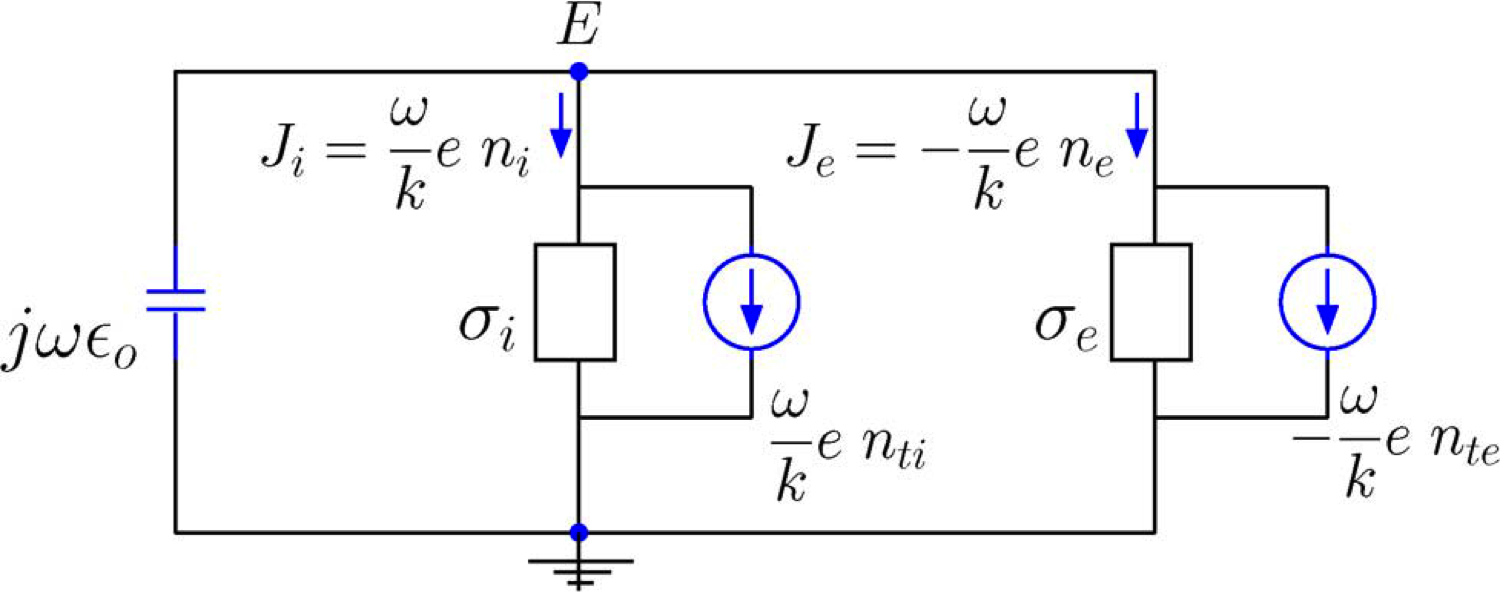
\includegraphics[width=3.0in]{circuit}
% where an .eps filename suffix will be assumed under latex, 
% and a .pdf suffix will be assumed for pdflatex; or what has been declared
% via \DeclareGraphicsExtensions.
\caption{Lumped circuit model seen in  \cite{kudeki:milla:1}.}
\label{fig:circuit}
\end{figure}

\noindent Using the electron current expression, $-\omega k^{-1}en_e = E\sigma_e -\omega k^{-1}en_{te}$, these equations can be rearranged to solve for $n_e$, 

\begin{equation}
\label{eq:neeq}
n_e(\mathbf{k},\omega) =  \frac{(j\omega\epsilon_0 + \sigma_i) n_{te}(\mathbf{k},\omega)}{j\omega\epsilon_0 +\sigma_e+\sigma_i} + \frac{\sigma_en_{ti}(\mathbf{k},\omega)}{j\omega\epsilon_0 +\sigma_e+\sigma_i}.
\end{equation}

\noindent To determine the power spectrum we square and average Equation \ref{eq:neeq} taking into account that the terms $n_{te}$ and $n_{ti}$ are independent of one and other we result in the following
\begin{equation}
\label{mainspeceq}
\langle \left|n_e(\mathbf{k},\omega)\right|^2\rangle = \frac{|j\omega\epsilon_0 + \sigma_i|^2 \langle |n_{te}(\mathbf{k},\omega)|^2\rangle}{|j\omega\epsilon_0 +\sigma_e+\sigma_i|^2} + \frac{| \sigma_e|^2 \langle |n_{ti}(\mathbf{k},\omega)|^2\rangle}{|j\omega\epsilon_0 +\sigma_e+\sigma_i|^2}.
\end{equation}

We can generalize them for multiple ion species by simply summing over the thermal fluctuations and conductances in Equation \ref{eq:ampscaler},

\begin{equation} 
\label{eq:ampscalersum}
0=\left(\displaystyle \sum_k^K\sigma_{ik} +\sigma_e\right)E +\frac{\omega}{k}e\left(\sum_k^Kn_{tik}-n_{te}\right) +j\omega \epsilon_0 E.
\end{equation}

\noindent This then augments the power spectrum in Equation \ref{mainspeceq} to the following

\begin{equation}
\label{eq:sumspeceq}
\displaystyle \langle \left|n_e(\mathbf{k},\omega)\right|^2\rangle = \frac{\left|j\omega\epsilon_0 +  \sum_k^K\sigma_{ik} \right|^2 \langle |n_{te}(\mathbf{k},\omega)|^2\rangle}{\left|j\omega\epsilon_0 +\sigma_e+ \sum_k^K\sigma_{ik} \right|^2} + \frac{| \sigma_e|^2 \left \langle \left|\sum_k^Kn_{tik}(\mathbf{k},\omega)\right|^2\right\rangle}{\left|j\omega\epsilon_0 +\sigma_e+ \sum_k^K\sigma_{ik} \right|^2}.
\end{equation}

%%%%%%%%%%%%%%%%%%%%%%%%%%%%%%%%%%%%%%%%%%%%%%%%%%%%%%%%%%%%%%%%%%%%%%
\section*{Gordeyeve Integrals}
The power spectrum of the thermal fluctuation for each species $s$ can be determined by the following,

\begin{equation}
\label{eq:thermalfl}
\frac{\langle|n_{ts}(\mathbf{k},\omega)|^2\rangle}{N_s} = 2\text{Re}\{J_s(\omega_s)\},
\end{equation}

\noindent where $N_s$ is the average density for the species.  Also the conductance for each species $s$ can be determine from the following,

\begin{equation}
\label{eq:cond}
\frac{\sigma_{s}(\mathbf{k},\omega)}{j\omega\epsilon_0} = \frac{1-j\omega_s J_s(\omega_s)}{k^2\lambda_s^2}
\end{equation}

\noindent where $\omega_s \equiv \omega-\mathbf{k}\cdot\mathbf{V}_s $ is the Doppler shifted frequency and $\lambda_s \equiv \sqrt{\frac{\epsilon_0 KT_s}{N_s q_s^2}}$ is the Debye length for each species.

The $J_s$ terms can be represented as follows

\begin{equation}
\label{eq:gord}
J_s(\omega)\equiv \int_0^\infty \langle e^{j\mathbf{k}\cdot\Delta \mathbf{r}_s}\rangle e^{j\omega\tau}d\tau
\end{equation}

\noindent These terms are known as Gordeyeve integrals, which are the one sided Fourier transforms of the characteristic functions of the particle displacements $\langle e^{j\mathbf{k}\cdot\Delta\mathbf{r}_s}\rangle$.  

The particle displacement function can change depending on magnetic field and collisionality of the plasma. For the high latitude F-region in the ionosphere a case of general importance is one of a non-magnitized and collision less plasma, where $\Delta\mathbf{r} = \mathbf{v}\tau$ where $\tau$ is the time interval. Assuming a Maxwellian the PDF of one dimensional displacement is

\begin{equation}
\label{eq:pdfr}
f(\Delta r) = \frac{1}{\sqrt{2\pi \langle r^2 \rangle}}e^{\frac{-\Delta r^2}{2\langle r^2\rangle}}.
\end{equation}
 
\noindent The variance term $\langle r^2 \rangle$ can be represented as
\begin{equation}
\label{eq:var}
\langle r^2 \rangle = \langle v^2 \rangle \tau^2 = \frac{KT_s}{m_s} \tau^2
\end{equation}
 \noindent where $T_s$ is the temperature of the species, $K$ is Boltzmans constant and $m_s$ is the mass of the species in kg. To simplify notation like in \cite{kudeki:milla:1}, we will refer to $\sqrt{KT_s/m_s}$ as $C$. Which yields the following single particle ACF,
 
 \begin{equation}
\label{eq:pdfall}
\langle e^{j\mathbf{k}\cdot\Delta \mathbf{r}}\rangle= e^{-\frac{1}{2}k^2C^2 \tau^2}.
\end{equation}
 
 To model collisions we use the term $\nu$ as the collision frequency for the species. If $\nu<<kC$ then \ref{eq:pdfall} can be used as the single particle ACF. If not the following must be used.
 
 \begin{equation}
 \label{eq:colspacf}
 \langle e^{j\mathbf{k}\cdot\Delta \mathbf{r}}\rangle = e^{-\frac{k^2C^2}{\nu^2}\left( \nu \tau-1+e^{-\nu\tau}\right)}
 \end{equation}
 
Lastly if one is to add a magnetic field to the equations the single particle ACFs must now take into a account the orientation of the magnetic field. The authors of \cite{kudeki:milla:1} use the convention of breaking up the Bragg vector $\mathbf{k}$ into two components, one parallel to the magnetic field, $k_{\parallel}$ and one perpendicular,$k_{\perp}$, as such, $\mathbf{k}= \hat{b}k_{\parallel}+\hat{p}k_{\perp}$. This yields the following formulation for the single particle ACF,

 \begin{equation}
\label{eq:pdfmag}
\langle e^{j\mathbf{k}\cdot\Delta \mathbf{r}}\rangle= e^{-\frac{1}{2}k_{\parallel}^2C^2 \tau^2}\times e^{-\frac{2k_{\perp}^2C^2}{\Omega^2} \sin^2(\Omega\tau/2)},
\end{equation}

\noindent where the gyro frequency is $\Omega = qB/m$This formulation neglects the effects of collisions which if taken into account yields the following single particle ACF,

\begin{equation}
\label{eq:colspacf}
\langle e^{j\mathbf{k}\cdot\Delta \mathbf{r}}\rangle = e^{-\frac{k_\parallel^2C^2}{\nu^2}\left( \nu \tau-1+e^{-\nu\tau}\right)}\times e^{-\frac{k_\perp^2C^2}{\nu^2+\Omega^2}\left(\cos(2\gamma) + \nu \tau-e^{-\nu\tau}\cos(\Omega\tau-2\gamma)\right)},
\end{equation}
 
\noindent where $\gamma = \tan^{-1}(\nu\Omega)$. The for the case with the magnetic field as one gets closer to being fulling perpendicular to $\mathbf{B}$ the single particle ACFs become much more narrow band, to the point of becoming delta functions in the frequency space. It is necessary to use other methods beyond numerical integration to determine the Gordeyeve Integrals. The authors of \cite{kudeki:milla:2} get around this problem by making a particle in cell simulation to determine the particle statistics. 


%%%%%%%%%%%%%%%%%%%%%%%%%%%%%%%%%%%%%%%%%%%%%%%%%%%%%%%%%%%%%%%%%%%%%%
 \section*{Computational Considerations}
One of the main challenges to calculating the ISR spectrums is calculating the Gordeyeve integrals. The case with no collisions or magnetic fields can be done analytically using Dawsons integral. This can be done using the identity

\begin{equation}
\label{eq:daw1}
jZ(\theta) = \int_0^{\infty} e^{-j\theta t}e^{-\frac{t^2}{4}}dt = \sqrt{\pi}e^{-\theta^2}-j2e^{-\theta^2}\int_0^\theta e^{t^2}dt.
\end{equation}

\noindent Using the terms found in Equation \ref{eq:pdfall}, $\theta=\omega_s/\left(\sqrt{2}kC\right)$ and $t=\sqrt{2}kC\tau$.

For other cases where analytical calculation is not possible a numerical integration scheme from \cite{Ooi:2007jx} is used. It is also possible to use a Chirp-z based algorithm that is shown in \cite{Li:1991gr} from the experiences of the author the first technique converges faster. The technique used in \cite{Ooi:2007jx} changes the variable of integration for integrals of the following form,

\begin{equation}
\label{eq:Sommer}
I=\int_a^b f(z) dz.
\end{equation}

\noindent The technique changes the variable $z$ in the following way,

\begin{equation}
\label{eq:newz}
z = \frac{1}{2}(a+b)+\frac{1}{2} (b-a)\text{Erf}(g(t)),
\end{equation}

\noindent where $g(t)$ is a function that is choosen so  $g(t)\rightarrow\pm \infty$ as $t\rightarrow\pm \infty$ and $Erf(u)$ is 
\begin{equation}
\label{eq:erf1}
\text{Erf}(u) = \frac{2}{\sqrt{\pi}}\int_0^u e^{-t^2}dt.
\end{equation}

\noindent Discretizing and changing variables the integral in Equation \ref{eq:Sommer} becomes the following sum

\begin{equation}
\label{eq:erfsum1}
I=\displaystyle \sum_{n=-N}^N A_nf\left( \frac{1}{2}(a+b)+\frac{1}{2} (b-a)\text{Erf}(g(nh))\right)
\end{equation}

\noindent where,
\begin{equation}
\label{eq:anterm}
A_n = g'(nh)e^{-g(nh)^2}.
\end{equation}

\noindent Like in \cite{Ooi:2007jx}, $g(nh) = \sinh (nh)$ and the grid spacing $h$ is the following,

\begin{equation}
\label{eq:hterm}
h = \frac{1}{N}\ln(1.05\sqrt{2}N).
\end{equation} 


Lastly to avoid cases of divid by zero errors the main equations have to be rearrange slightly. First off because some ion species could have zero density Equation \ref{eq:cond} uses the Debye length of the electron species,$\lambda_e$ as follows

\begin{equation}
\label{eq:condnew}
\frac{\sigma_{s}(\mathbf{k},\omega)}{j\omega\epsilon_0} = \frac{1-j\omega_s J_s(\omega_s)}{k^2\lambda_e^2} \left(\frac{q_sT_eN_s}{q_eT_sN_e}\right).
\end{equation}

Also, to avoid having to more calculations then necessary the $j\omega\epsilon_0$. terms of Equation \ref{eq:sumspeceq} are moved around. Thus it becomes,

\begin{equation}
\label{eq:sumspeceqfinal}
\displaystyle \langle \left|n_e(\mathbf{k},\omega)\right|^2\rangle =  \frac{\left|1 +  \sum_k^K\frac{\sigma_{ik}}{j\omega\epsilon_0} \right|^2 \langle |n_{te}(\mathbf{k},\omega)|^2\rangle}{\left|1 +\frac{\sigma_e+ \sum_k^K\sigma_{ik}}{j\omega\epsilon_0} \right|^2} + \frac{\left| \frac{\sigma_e}{j\omega\epsilon_0} \right|^2\left \langle \left|\sum_k^Kn_{tik}(\mathbf{k},\omega)\right|^2\right\rangle}{\left|1 +\frac{\sigma_e+ \sum_k^K\sigma_{ik}}{j\omega\epsilon_0} \right|^2}.
\end{equation}

\noindent If the Gordeyeve integrals are substitute in Equation \ref{eq:sumspeceqfinal} it becomes the following.

\begin{equation}
\label{eq:sumspeceqactual}
\begin{split}
\displaystyle \langle \left|n_e(\mathbf{k},\omega)\right|^2\rangle =&  \frac{\left|1 + \sum_s^K  \frac{1-j\omega_s J_s(\omega_s)}{k^2\lambda_e^2} \left(\frac{q_sT_eN_s}{q_eT_sN_e}\right) \right|^2 2N_e\text{Re}\{J_e(\omega_e)\}}{\left|1 + \frac{1-j\omega_e J_e(\omega_e)}{k^2\lambda_e^2}  +\sum_s^K  \frac{1-j\omega_s J_s(\omega_s)}{k^2\lambda_e^2} \left(\frac{q_sT_eN_s}{q_eT_sN_e}\right) \right|^2}       + \\        & \frac{\left| \frac{1-j\omega_s J_e(\omega_e)}{k^2\lambda_e^2} \right|^2\sum_s^K  2N_s\text{Re}\{J_s(\omega_s)\}}{\left|1 + \frac{1-j\omega_e J_e(\omega_e)}{k^2\lambda_e^2}  +\sum_s^K  \frac{1-j\omega_s J_s(\omega_s)}{k^2\lambda_e^2} \left(\frac{q_sT_eN_s}{q_eT_sN_e}\right) \right|^2}.
\end{split}
\end{equation}

\section*{Examples}
We can see in Figure \ref{fig:diffspectrums} examples of ISR spectrums from different ISR systems. The spectrums were generated using the the parameters values $N_e=1\times10^{11}$, $T_e=3000^o$K and $T_i=3000^o$K and the system parameter values seen in Table \ref{tab:ISRsys}. The ion acoustic frequency$f_{ia}$ for each system with the following plasma parameters its wavelength $\lambda$ was calculated using the following formula,

\begin{equation}
\label{eq:iaf}
f_{ia} = \frac{\lambda}{2}\sqrt{\frac{k_bT_e +k_b\gamma_iT_i}{M}},
\end{equation}

\noindent where $M$ is the ion mass in kg, $k_b$ is Botlzmann's constant and $\gamma_i$ is the adiabatic index which is set to 3 in all cases. In most of the cases the familiar double hump spectrum is visible. The only exception to this is Jicamarca, where the system's k-vector is very close to being perpendicular to the earths magnetic field. This also impacts the amount of time it takes to calculate the spectrum because as the k-vector gets closer to being perpendicular to magnetic field the Gordeyeve integral will take longer to converge.
\begin{figure}[!h]
\centering
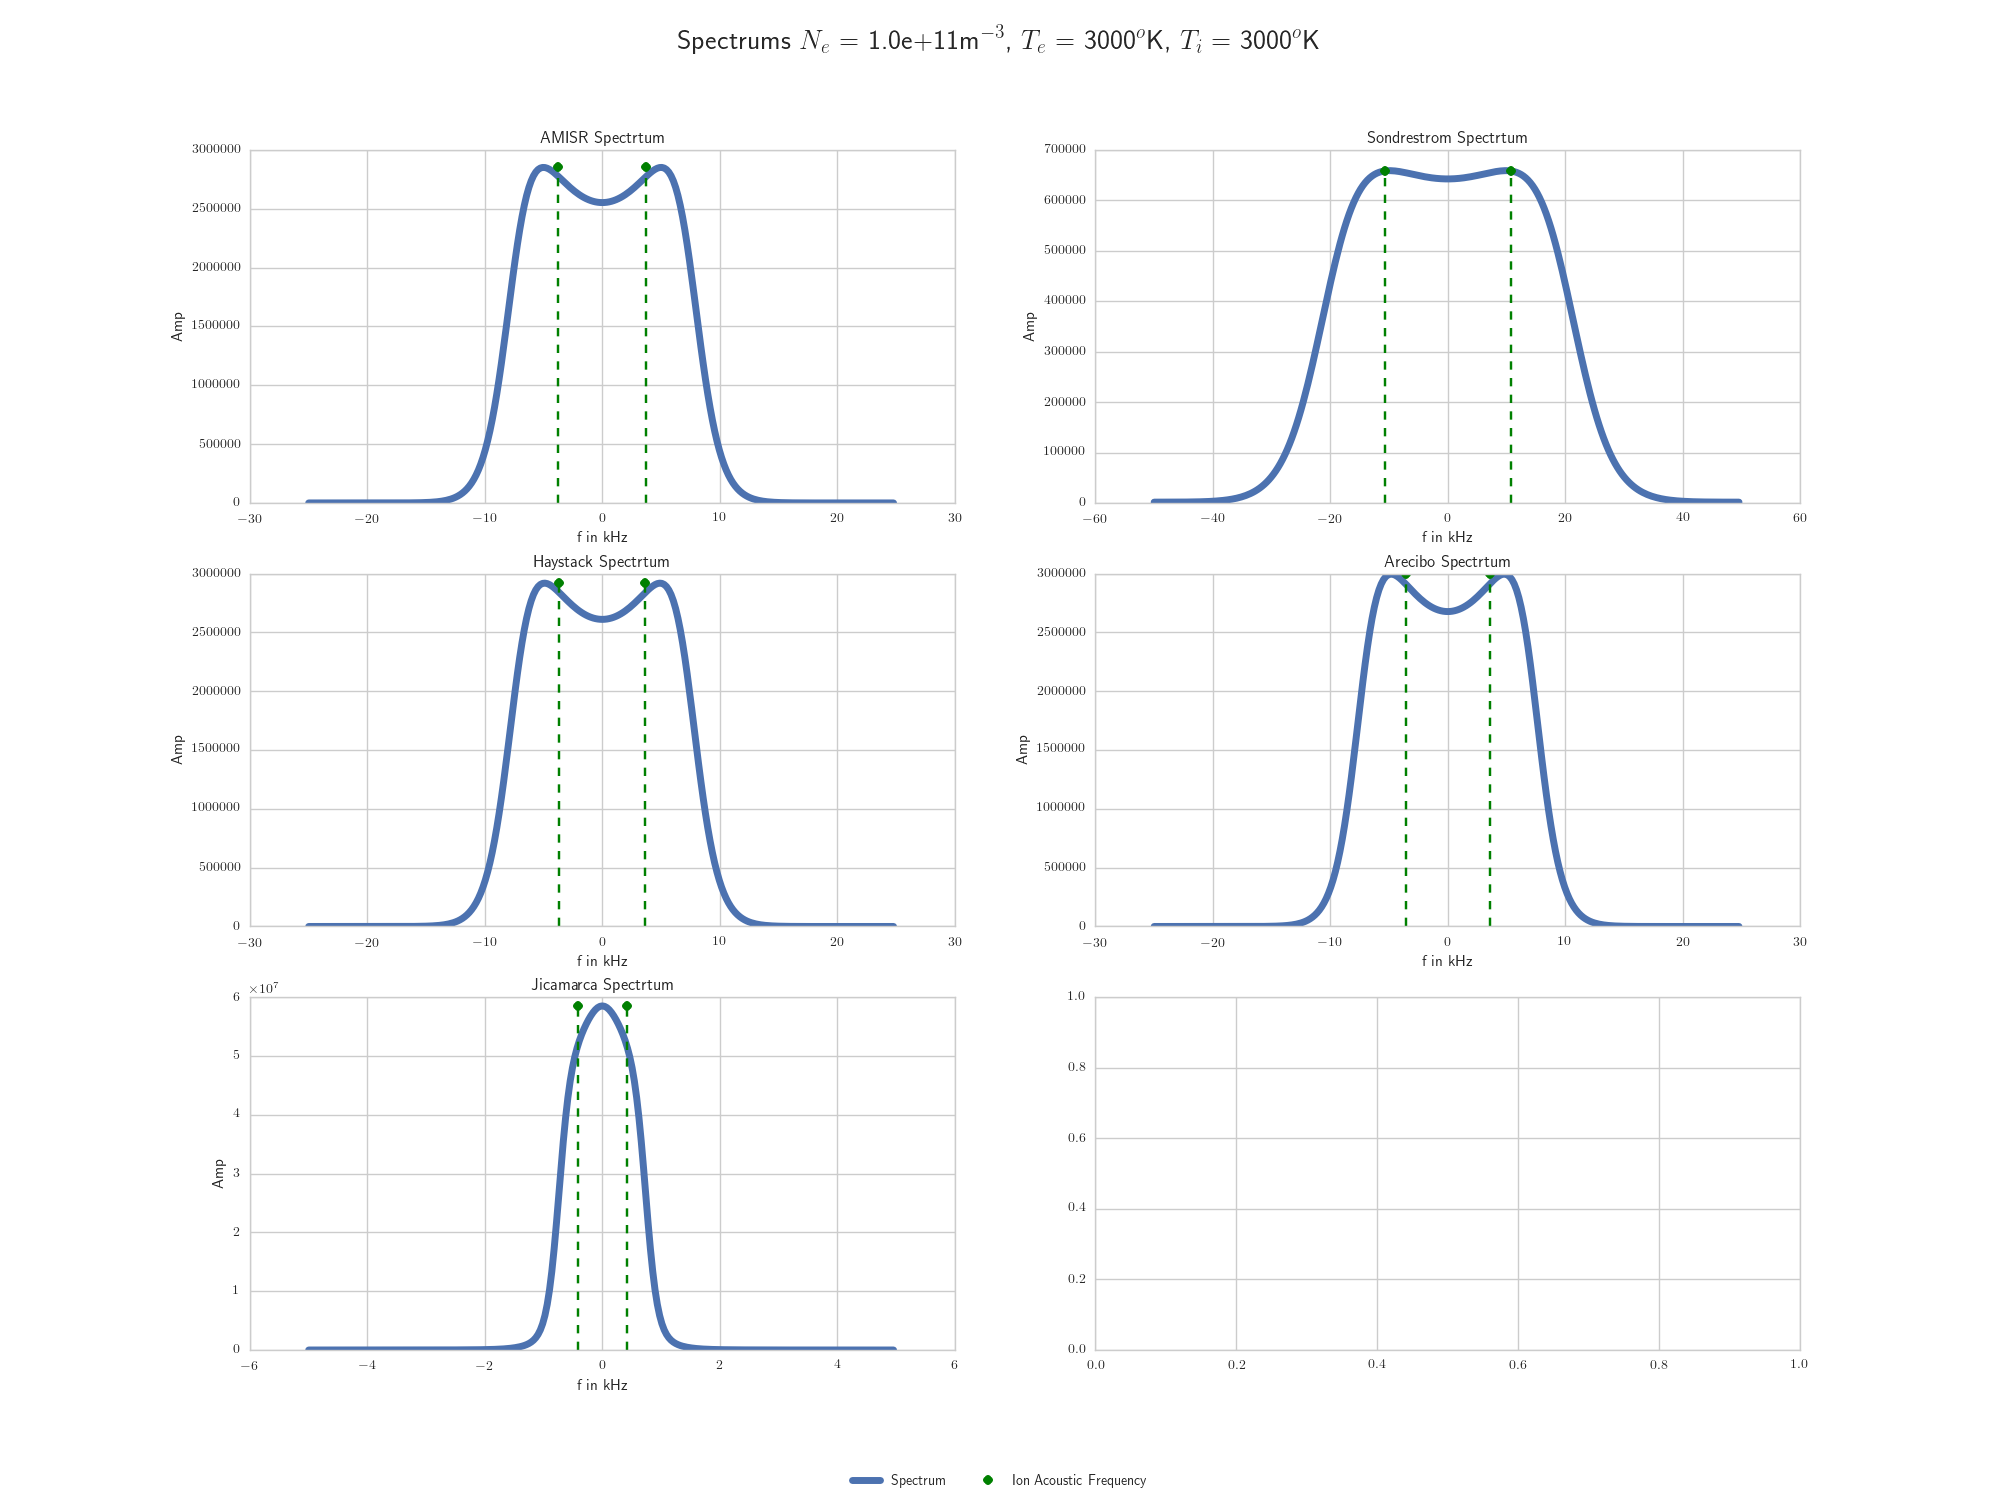
\includegraphics[width=7.0in]{DifferentSystems}

\caption{Spectrums From Different ISR Systems}
\label{fig:diffspectrums}
\end{figure}


\begin{table}[!h]
\centering
\caption{ISR System Parameters}
\label{tab:ISRsys}
\begin{tabular}{lllll}
System Name & $f_0$ in MHz & $f_s$ in kHz & $\alpha$ in $^o$ &  \\
AMISR       & 449          & 50           & 70               &  \\
Sondrestrom & 1290         & 100          & 80               &  \\
Haystack    & 440          & 50           & 65               &  \\
Arecibo     & 430          & 50           & 45               &  \\
Jicamarca   & 50           & 10           & 1                & 
\end{tabular}
\end{table}
\end{appendices}
%==========================================================================%
% Bibliography
\newpage
\singlespace
\bibliographystyle{apalike}

% each subdirectory can have its own BiBTeX file
\bibliography{BibTex/litreview.bib}
\cleardoublepage

%==========================================================================%
% Curriculum Vitae
\addcontentsline{toc}{chapter}{Curriculum Vitae}

\thispagestyle{empty}

\begin{center}
{\LARGE {\bf CURRICULUM VITAE}}\\
\vspace{0.5in}
{\large {\bf John Swoboda}}
\end{center}

\section*{EDUCATION}{\sl PhD,} Electrical Engineering, Fall 2016; Expected \\
                      % \sl will be bold italic in New Century Schoolbook (or
	              % any postscript font) and just slanted in
		      %	Computer Modern (default) font
                GPA 3.90/4.00 \\
                Boston University, Boston, MA
	       

{\sl Master of Science,} Electrical Engineering, May 2008 \\
                      % \sl will be bold italic in New Century Schoolbook (or
	              % any postscript font) and just slanted in
		      %	Computer Modern (default) font
                 GPA 3.71/4.00\\
                Thesis Title: Reconstruction of Tomographic Images Corrupted by a Slice Sensitivity Profile With Applications to The Inspection of Manufactured Items\\
 {\sl Bachelor of Science,} Electrical \& Computer Systems Engineering, May 2007  \\
                GPA: 3.74/4.00\\
                Rensselaer Polytechnic Institute, Troy, NY, \\
                
 
 

 
\section*{RELEVENT \\ EXPERIENCE}
 {\sl Research Assistant} \hfill            September 2012 - Present \\
                Electrical Engineering Department, Boston University 
                 \begin{itemize}  \itemsep -2pt %reduce space between items
                 \item Performed data fusion and analysis from varied sensor types for geophysical research.
                 \item Created theoretical frame work for incoherent scatter radar data processing.
                 \item Developed simulations, algorithms for incoherent scatter radar systems.
                 \end{itemize} 

 {\sl Sensor System Engineer} \hfill January 2009 - August 2012\\
                The MITRE Corporation, Bedford MA 
                 	\begin{itemize}  \itemsep -2pt %reduce space between items
                	\item Developed new algorithms for experimental radar systems.
                	\item Created full signal processing level emulations and simulations of radar systems.
                \end{itemize}
 
                {\sl Research Assistant} \hfill            May 2009 - January 2009 \\
                Electrical Engineering Department, Rensselaer Polytechnic Institute 
                 \begin{itemize}  \itemsep -2pt %reduce space between items
                 \item Developed signal processing algorithms applied to image formation radar.
                 \end{itemize} 
                {\sl Research Engineering Intern} \hfill        May 2007 - May 2008\\
                Lickenbrock Technologies, Troy NY
                  \begin{itemize}
                   \item Developed signal processing algorithms for the deblurring of tomographic images.
                   \end{itemize} 
\section*{COMPUTER \\ SKILLS} {\sl Languages \& Software:} Python, MATLAB, C, C$++$, \LaTeX, Git, Microsoft Office.\\
                {\sl Operating Systems:} Mac OS X, Linux, Windows. 
 
\section*{PUBLICATIONS}   

\begin{itemize}
	\item Swoboda, J., Semeter J., Improvement of Resolution of Incoherent Scatter Radar Using Electronically Scanned Arrays and Inverse Theory, IEEE Symposium on Phased Array Technology, 2016
	\item Swoboda, J., Semeter J., Erickson, P., Zettergren M., Observability of Ionospheric Space-Time Structure with ISR:   A Simulation Study, (To be Submitted). 
	\item Swoboda, J., J. Semeter, and P. Erickson (2015), Space-time ambiguity functions for electronically scanned ISR applications, Radio Sci., 50, 2015. DOI: 10.1002/2014RS005620

	\item Krishnan, V., Swoboda, J., Yarman, C.E., Yazici, B. , Multistatic Synthetic Aperture Radar Image Formation, IEEE Transactions on Image Processing , vol.19, no.5, pp.1290-1306, May 2010
    \item  Swoboda, J., Yarman, C. E., Yazici, B., Bistatic synthetic aperture radar imaging for arbitrary trajectories in the presence of noise and clutter. Proc. SPIE 7307, Airborne Intelligence, Surveillance, Reconnaissance (ISR) Systems and Applications VI, 73070D April 28, 2009 
\end{itemize}
	
\section*{PRESENTATIONS}
\begin{itemize}
	\item Swoboda, J., Hirsch, M.,Semeter, J., GeoData Python Toolset: High Performance Python for Geoscience, CEDAR Workshop, 2016
    \item Swoboda, J.,  Semeter, J., The "Impulse Response" of Electronically Scanned and Dish Based ISR, URSI, 2016
    \item Swoboda, J., Semeter J., Erickson, P., Zettergren M., Impact of the Forward Model of ESA Based ISR on Measurements from HAARP, CEDAR, 2015
	\item Swoboda, J., Semeter J., Erickson, P., Zettergren M., Three Dimensional Ionosphere Reconstruction from Electronically Steerable ISR, MTSSP, 2015
	\item Swoboda, J., Dahlgren, H., Semeter J., Erickson, P., On the Way to Optimal Processing for Multi-beam RISR Experiments, CEDAR, 2014
    \item Swoboda, J., Semeter J., Erickson, P., Simulation of ISR Data and Application to Spatial Sampling of the Ionosphere, URSI, 2015
\end{itemize}

\section*{POSTER \\ PRESENTATIONS}
\begin{itemize}
\item Swoboda, J., Semeter J., Improvement of Resolution of Incoherent Scatter Radar Using Electronically Scanned Arrays and Inverse Theory, NEROC Symposium, 2016
\item Swoboda, J., Semeter J., Improvement of Resolution of Incoherent Scatter Radar Using Electronically Scanned Arrays and Inverse Theory, IEEE Symposium on Phased Array Technology, 2016
\item Swoboda, J.,  Semeter, J., Resolving Cross Range Gradients in the High Latitude Ionosphere, CEDAR Workshop, 2016
\item Swoboda, J., Hirsch, M.,Semeter, J., GeoData: A Generalized Data Analysis Software Suite, CEDAR Workshop, 2015
\item Swoboda, J., Dahlgren, H., Semeter J., Erickson, P., Plasma Motion Induced Artifacts in 3-D Incoherent Scatter Radar, CEDAR, 2014
\end{itemize}

\section*{CODE / DATASETS}
\begin{itemize}
\item J. Swoboda, M. Hirsch, A. Stuhlmacher, G. Starr, and Semeter, J. (2016). GeoData Python [code]. Zenodo. http://doi.org/10.5281/zenodo.154533
\end{itemize}
 

%==========================================================================%
\end{document}
